\documentclass[a4paper,14pt]{extreport}

\usepackage[english,ukrainian]{babel}
\usepackage[top=20mm,bottom=20mm,left=25mm,right=15mm,headsep=6mm]{geometry}
\usepackage{amsmath, hyperref, array, multirow}
\usepackage[T1]{fontenc}
\usepackage{appendix}
\usepackage{float}

%\usepackage{showframe}
%\usepackage[demo]{graphicx}
\usepackage{graphicx}

\graphicspath{{figures/}}

\newcolumntype{P}[1]{>{\hspace{0pt}\centering\arraybackslash}p{#1}}
\newcolumntype{M}[1]{>{\hspace{0pt}\centering\arraybackslash}m{#1}}

\addto\captionsukrainian{\renewcommand{\figurename}{Рисунок}}

\usepackage{titlesec, placeins}
\usepackage{etoolbox}
% \titlespacing{<command>}{<left>}{<before-sep>}{<after-sep>}[<right>]
% \titleformat{⟨command⟩}[⟨shape⟩]{⟨format⟩}{⟨label⟩}{⟨sep⟩}{⟨before-code⟩}[⟨after-code⟩]


% \titleformat{\chapter}[display] {\centering\MakeUppercase}{\chaptername\ \thechapter\ }{\ }{\Huge\textbf}

%\titlespacing{\chapter} {0pt}{50pt}{1pt}

% FIX: Chapters should be in titlecase just like in the TOC
\titleformat{\chapter}
{\centering\MakeUppercase} % format
{\chaptername\ \thechapter\ } % label РОЗДІЛ 1
{0pt}
{}

\titlespacing{\chapter}
{0pt}
{-\topskip}
{\baselineskip}

% FIX: Make the right spacing between sections and figures/lists as par with the right spacing between the chapter title and page header. Use \\ if the title overlaps the preceding text
\titleformat{\section}{\centering\MakeUppercase}{\thesection\ }{0pt}{}
\titlespacing{\section}{0pt}{-\topskip}{\baselineskip}

\titleformat{\subsection}{\centering\MakeUppercase}{\thesubsection\ }{0pt}{}
\titlespacing{\subsection}{0pt}{-\topskip}{\baselineskip}

%\let\Oldsection\section
%\renewcommand{\section}{\FloatBarrier\Oldsection}

%\let\Oldchapter\chapter
%\renewcommand{\chapter}{\FloatBarrier\Oldchapter}

\usepackage{titletoc}
\makeatletter

% \titlecontents{⟨section⟩}[⟨left⟩]{⟨above-code⟩}
% {⟨numbered-entry-format⟩}{⟨numberless-entry-format⟩}
% {⟨filler-page-format⟩}[⟨below-code⟩]

% FIX: Chapters should be in titlecase
\titlecontents{chapter}
[0pt]                     % left margin
{}                        % formatting before
{\bfseries\MakeUppercase\@chapapp\ \thecontentslabel.\ \MakeUppercase} % numbered format
{\bfseries\MakeUppercase} % numberless format
{\bfseries\titlerule*[0.5pc]{.}\contentspage} % filler
{}                        % formatting after

% \titlecontents{chapter}[0pt]{}{\bfseries\@chapapp\ \thecontentslabel.\ }{\bfseries}{\bfseries\titlerule*[0.5pc]{.}\contentspage}{}

\titlecontents{section}
[12mm]                               % left margin
{}
{\thecontentslabel.\hspace{0.3em}}   % numbered format
{}
{\titlerule*[0.5pc]{.}\contentspage} % filler
{}

\titlecontents{subsection}
[\dimexpr12mm+1.8em\relax]           % left margin
{}
{\thecontentslabel.\hspace{0.3em}}   % numbered format
{}
{\titlerule*[0.5pc]{.}\contentspage} % filler
{}

% РОЗДІЛ А Додаток 1 -> ДОДАТОК А\nДодаток 1
\g@addto@macro\appendices{
  \addtocontents{toc}{\protect\renewcommand{\protect\@chapapp}{\appendixname}}
  \titleformat{\chapter}[display] {\centering}
    {\MakeUppercase{\appendixname}\enspace\thechapter}
    {.5em}
    {\centering\MakeUppercase}
}
\makeatother


% for diploma and courseworks
\usepackage{chngcntr}
\addto\captionsukrainian{\renewcommand{\abstractname}{Реферат}}

\newenvironment{abstractpage}
  {\addcontentsline{toc}{chapter}{Реферат}
  \cleardoublepage\vspace*{\fill}
  \thispagestyle{empty}}
  {\cleardoublepage}

\renewenvironment{abstract}[1]
    {\selectlanguage{#1}
    \begin{center}\MakeUppercase\abstractname\end{center}}
    {\par\vfill}

\usepackage[autostyle]{csquotes}
%\usepackage{url}
\usepackage{soul}
\usepackage[
  backend=biber,
  bibencoding=utf8,
  hyperref=auto,
  sorting=ntvy,
  language=auto,
  autolang=other,
  style=gost-numeric,
  url=false
]{biblatex}

\renewcommand*{\mkgostheading}[1]{#1}
%\renewcommand*{\newblockpunct}{\addperiod\space\bibsentence}
\renewcommand*{\addcolondelim}{\addcolon\space}

%\urlstyle{same}

% TODO: make urls prettier

\usepackage{hyperref}
\hypersetup{
    breaklinks=true,
    hidelinks, % Remove visible links altogether
    %urlbordercolor = 1 1 1% Make URL link border white
}
\DeclareFieldFormat{url}{URL:~\href{#1}{\ul{#1}}}

% \usepackage{xcolor}
% \usepackage{hyperref}
% \hypersetup{
%     breaklinks=true,
%     hidelinks,
%     allbordercolors=black,
%     pdfborderstyle={/S/U/W 1},
% }
% \DeclareFieldFormat{url}{URL:~\url{#1}}

\renewcommand\UrlFont{\rmfamily}

\nocite{*}

\addbibresource{bibliography.bib}

\usepackage{xassoccnt}
\usepackage{lastpage}

\NewTotalDocumentCounter{totalfigures}
\NewTotalDocumentCounter{totaltables}
\NewTotalDocumentCounter{totallistings}
\NewTotalDocumentCounter{appendixchapters}
\DeclareAssociatedCounters{figure}{totalfigures}
\DeclareAssociatedCounters{table}{totaltables}
\DeclareAssociatedCounters{lstlisting}{totallistings}

\NewTotalDocumentCounter{totalbibliography}
\AtDataInput{{\stepcounter{totalbibliography}}{}}


\usepackage{fontspec}
\usepackage[english,ukrainian]{babel}
\setmainfont[]{Times New Roman}

\usepackage{setspace}
\onehalfspacing
\setlength{\parindent}{1.25cm}

\tolerance=1
\emergencystretch=\maxdimen
% \hyphenpenalty=10000 % should be commented if using lualatex
\hbadness=10000

% \sloppy

\usepackage{ragged2e}
\justifying

\usepackage{enumitem}
\setlist{nosep, after=\vspace{8pt}, before=\vspace{8pt}, leftmargin=1.26cm, itemsep=1mm, labelsep=0.63cm, itemsep=6pt}

% make dashes default for itemize
\renewcommand\labelitemi{--}

\newcommand{\defaultenumsep} {\setlist{nosep, after=\vspace{\baselineskip}, before=\vspace{8pt}, itemsep=8pt}}

\usepackage{fancyhdr}

% headings is a default style for sections and subsections
\fancypagestyle{headings}{
    \renewcommand{\headrulewidth}{0pt}
    \fancyhf{}
    \fancyhead[R]{\thepage}
}

% plain is a default style for chapters
\fancypagestyle{plain}{
    \renewcommand{\headrulewidth}{0pt}
    \fancyhf{}
    \fancyhead[R]{\thepage}
}


\usepackage{listings}

\lstset{upquote=true}

% straight double quotes hack
\makeatletter
\lst@CCPutMacro
    \lst@ProcessOther {"22}{\lst@ifupquote \textquotedbl
                                     \else \char34\relax \fi}
    \@empty\z@\@empty
\makeatother

% Значения по умолчанию
\lstset{
  basicstyle=\footnotesize,
  breakatwhitespace=true,% разрыв строк только на whitespacce
  breaklines=true,       % переносить длинные строки
%   captionpos=b,          % подписи снизу -- вроде не надо
  inputencoding=koi8-r,
  numbers=left,          % нумерация слева
  numberstyle=\footnotesize,
  showspaces=false,      % показывать пробелы подчеркиваниями -- идиотизм 70-х годов
  showstringspaces=false,
  showtabs=false,        % и табы тоже
  stepnumber=1,
  xleftmargin=2em,
  tabsize=4,              % кому нужны табы по 8 символов?
  frame=single,
  escapeinside={(/}{/)},
  otherkeywords={\&},
  emph={&},
}

% correctly render cyrillic comments
\makeatletter
\lst@InputCatcodes
\def\lst@DefEC{%
    \lst@CCECUse \lst@ProcessLetter
    ^^^^0410^^^^0411^^^^0412^^^^0413^^^^0490^^^^0414^^^^0415^^^^0404% А Б В Г Ґ Д Е Є
    ^^^^0416^^^^0417^^^^0418^^^^0406^^^^0407^^^^0419^^^^041a^^^^041b% Ж З И І Ї Й К Л
    ^^^^041c^^^^041d^^^^041e^^^^041f^^^^0420^^^^0421^^^^0422^^^^0423% М Н О П Р С Т У
    ^^^^0424^^^^0425^^^^0426^^^^0427^^^^0428^^^^0429^^^^042c^^^^042e% Ф Х Ц Ч Ш Щ Ь Ю
    ^^^^042f% Я
    ^^^^0430^^^^0431^^^^0432^^^^0433^^^^0491^^^^0434^^^^0435^^^^0454% а б в г ґ д е є
    ^^^^0436^^^^0437^^^^0438^^^^0456^^^^0457^^^^0439^^^^043a^^^^043b% ж з и і ї й к л
    ^^^^043c^^^^043d^^^^043e^^^^043f^^^^0440^^^^0441^^^^0442^^^^0443% м н о п р с т у
    ^^^^0444^^^^0445^^^^0446^^^^0447^^^^0448^^^^0449^^^^044c^^^^044e% ф х ц ч ш щ ь ю
    ^^^^044f% я
    ^^^^042a^^^^042b^^^^042d% Ъ Ы Э
    ^^^^044a^^^^044b^^^^044d% ъ ы э
    ^^00}
\lst@RestoreCatcodes
\makeatother

% Стиль для псевдокода: строчки обычно короткие, поэтому размер шрифта побольше
\lstdefinestyle{pseudocode}{
  basicstyle=\small,
  keywordstyle=\color{black}\bfseries\underbar,
  language=Pseudocode,
  numberstyle=\footnotesize,
  commentstyle=\footnotesize\it
}

% Стиль для обычного кода: маленький шрифт
\lstdefinestyle{realcode}{
  basicstyle=\scriptsize,
  numberstyle=\footnotesize
}

% Стиль для коротких кусков обычного кода: средний шрифт
\lstdefinestyle{simplecode}{
  basicstyle=\footnotesize,
  numberstyle=\footnotesize
}

\lstdefinestyle{csharp}{language=[Sharp]C, style=simplecode}
\lstdefinestyle{csharp-small}{language=[Sharp]C, style=realcode}
\lstdefinestyle{cpp-small}{language=C++, style=realcode}

\usepackage{caption}

\DeclareCaptionLabelSeparator{custom}{ -- }
\captionsetup {
    labelsep=custom
}

%\captionsetup{labelsep=emdash,aboveskip=10pt,belowskip=0pt,position=bottom}

% У рисунков вырвнивание по центру
%\captionsetup[figure]{justification=centering}
% У таблиц -- слева, зазор 5pt вместо 10
%\captionsetup[table]{position=top,aboveskip=5pt}

\captionsetup{aboveskip=10pt,belowskip=0pt,position=bottom}
\captionsetup[table]{position=top, singlelinecheck=off, aboveskip=5pt}
\captionsetup[lstlisting]{position=top, singlelinecheck=off, margin=1.5em, font=small}

\newcommand*{\Topic}[1] {\textbf{Тема:} #1}
\newcommand*{\Purpose}[1] {\textbf{Мета:} #1}
\newcommand*{\Variant}[1] {\textbf{Варіант:} \textnumero#1}

\newcommand*{\Introduction} {
    \pagestyle{headings}
    \chapterhere*[headings]{Вступ}
    \addcontentsline{toc}{chapter}{Вступ}
}
\newcommand*{\TaskList} {
    \chapterhere*{Завдання}
    \addcontentsline{toc}{chapter}{Завдання}
    \thispagestyle{empty}
}
\newcommand*{\Conclusion} {
    \chapterhere*[headings]{Висновки}
    \addcontentsline{toc}{chapter}{Висновки}
}
\newcommand*{\FirstChapter}[1] {
    \pagestyle{headings}
    \chapter{#1}
    \thispagestyle{headings}
}
\newcommand*{\toc} {
    \phantomsection
    \addcontentsline{toc}{chapter}{Зміст}
    %\addtocontents{toc}
    %{\protect\thispagestyle{empty}}
    \tableofcontents
    \thispagestyle{empty}
    \clearpage
}

\newcommand*{\hyp}[1] {
    \fussy\hyphenpenalty=50\hbadness=1000
    #1
}

\NewDocumentCommand{\chapterhere}{s o m }{%
    \begingroup
    \let\clearpage\relax
    \IfBooleanTF{#1}
      {\chapter*{#3}}
      {\chapter{#3}}
    \IfValueTF{#2}
        {\thispagestyle{#2}}
        {}
    \endgroup
}


\title{курсового проєкту}
% \title{лабораторної роботи}

\author{АВТОР}
\def\Subject{%
    ДИСЦИПЛІНА\ignorespaces
}
\def\CourseYear{%
    КУРС
}
\def\StudGroup{%
    ГРУПА
}
\def\Mentor{%
    ХТО ПЕРЕВІРИВ/КЕРІВНИК\ignorespaces
}


\begin{document}

\makeatletter
\begin{titlepage}
    \begin{center}
        МІНІСТЕРСТВО ОСВІТИ І НАУКИ УКРАЇНИ\\
        НАЦІОНАЛЬНИЙ ТЕХНІЧНИЙ УНІВЕРСИТЕТ\\
        <<ХАРКІВСЬКИЙ ПОЛІТЕХНІЧНИЙ ІНСТИТУТ>>\\
        \vspace*{\baselineskip}
        \raggedright
        Інститут \underline{комп'ютерних наук та інформаційних технологій}\\
        Кафедра \underline{комп’ютерної інженерії та програмування}\\
        Спеціальність \underline{123 Комп’ютерна інженерія}\\
        Освітня програма \small \setstretch{1.5} \underline{Сучасне програмування, мобільні пристрої та комп'ютерні ігри}

        \vspace*{3\baselineskip}
        \normalsize
        \centering
        \onehalfspacing

        ПОЯСНЮВАЛЬНА ЗАПИСКА\\
        до \@title\\
        з навчальної дисципліни: ``\Subject''\\

        \vspace*{3\baselineskip}
        \raggedleft

        \begin{minipage}{0.58\textwidth}
            \raggedleft
            Виконав студент \CourseYear курсу, групи \StudGroup\\
            \vspace{0.3\baselineskip}

            \underline{\hspace{2cm}} / \@author/\\
            {\scriptsize (підпис, прізвище та ініціали)}
            
            \vspace*{\baselineskip}

            \begin{minipage}{0.58\textwidth}
                \begin{tabular}{@{}ll}
                 Керівник: & \\
                 к.ф.-м., проф. &\\
                \end{tabular}
            \end{minipage}
            \vspace{0.3\baselineskip}
            
            \underline{\hspace{2cm}} / \Mentor/\\
            {\scriptsize (підпис, прізвище та ініціали)}

            \vspace*{0.5\baselineskip}

            \begin{minipage}{0.58\textwidth}
                \begin{tabular}{@{}ll}
                 Нормконтроль: & \\
                 к.ф.-м., проф. &\\
                \end{tabular}
            \end{minipage}
            \vspace{0.3\baselineskip}
            
            \underline{\hspace{2cm}} / \Mentor/\\
            {\scriptsize (підпис, прізвище та ініціали)}
        \end{minipage}

        \centering
        \vfill
        Харків \the\year
    \end{center}
\end{titlepage}
\makeatother
\setcounter{page}{2}
% \pagestyle{empty}


% Regular labs
% \makeatletter
\begin{titlepage}
    \begin{center}
        МІНІСТЕРСТВО ОСВІТИ І НАУКИ УКРАЇНИ\\
        НАЦІОНАЛЬНИЙ ТЕХНІЧНИЙ УНІВЕРСИТЕТ\\
        <<ХАРКІВСЬКИЙ ПОЛІТЕХНІЧНИЙ ІНСТИТУТ>>\\
        \vspace*{\baselineskip}
        \raggedright
        Інститут \underline{комп'ютерних наук та інформаційних технологій}\\
        Кафедра \underline{комп’ютерної інженерії та програмування}\\
        Спеціальність \underline{123 Комп’ютерна інженерія}\\
        Освітня програма \small \setstretch{1.5} \underline{Сучасне програмування, мобільні пристрої та комп'ютерні ігри}

        \vspace*{3\baselineskip}
        \normalsize
        \centering
        \onehalfspacing

        ЗВІТ\\
        з \@title\\
        з навчальної дисципліни:\\
        ``\Subject''\\

        \vspace*{3\baselineskip}
        \raggedleft

        \begin{minipage}{0.58\textwidth}
            \raggedleft
            Виконав студент \CourseYear курсу, групи \StudGroup\\
            \vspace{0.3\baselineskip}

            \underline{\hspace{2cm}} / \@author/\\
            {\scriptsize (підпис, прізвище та ініціали)}
            
            \vspace*{0.5\baselineskip}

            \begin{minipage}{0.58\textwidth}
                \begin{tabular}{@{}ll}
                 Перевірив: & \\
                \end{tabular}
            \end{minipage}
            \vspace{0.3\baselineskip}
            
            \Mentor\\
            {\scriptsize (прізвище та ініціали)}
        \end{minipage}

        \centering
        \vfill
        Харків \the\year
    \end{center}
\end{titlepage}
\makeatother
\setcounter{page}{2}
\pagestyle{empty}

% \Topic{ТРИГЕРИ}
\Purpose{розглянути принципи побудови тригерів.}
\Variant{15}
\newline


\TaskList
\vspace{-\topsep}

Розробити пристрій на базі мікроконтролера Atmega328p, для порівняння аналогових та цифрових датчиків температури, з можливістю перемикання між ними у реальному часі із виводом температури на LCD дисплей типу Hitachi HD44780.

Зробити виміри у різних середовищах, побудувати відповідні графіки та порівняти результати з теоретичними характеристиками обраних датчиків.

\clearpage

\begin{abstractpage}
    \begin{abstract}{ukrainian}
        \par
        % FIX: page counter should stop at appendices as per DSTU
        Звіт про КР: \pageref{LastPage} с., \TotalValue{totaltables} табл., \TotalValue{totalfigures} рис., \TotalValue{totallistings} ліст., \TotalValue{appendixchapters} дод., \thetotalbibliography\ джерел.
        
        \bigskip
        \MakeUppercase{Atmega328p, датчики, термістор, термопара, NTC, DS18B20, DHT11, DHT22, HTU21D, цифрові, аналогові, proteus}
        \bigskip

        \textbf{Об'єкт дослідження} -- цифрові та аналогові датчики температури.
        
        \textbf{Метою} цієї роботи порівняння характеристик аналогових та цифрових датчиків температури, а також розробка програми для їх інтеграції з мікроконтролером.

        \textbf{Актуальність} роботи полягає у тому, що в сучасному світі неможливо розробляти електронні пристрої, не вимірюючи, при цьому температури їхнього мікропроцесора, нагрівального елементу, пристроїв збереження інформації (жорстких та SSD дисків), а також, профільних рішень клімат-контролю та ``розумної'' теплиці. А отже, потрібно вибирати правильні датчики, в залежності від вимог продукту.

        \textbf{Структура роботи}. Пропонована курсова робота складається із вступу, двох розділів -- теоретичної (вибір датчиків та їх загальний огляд) та практичної частини (проєктування схеми у САПР Proteus, написання програми та збірка реального макету, графіки), висновків до кожної з них, загальних висновків та списку літератури.

        Було зібрано пристрій, на базі Arduino UNO R3, до
        якого під'єднано декілька найцікавіших, на мій погляд, датчиків. Уся
        інформація виводитися на LCD дисплей, дані для графіків
        відправляти за допомогою Serial інтерфейсу на комп'ютер, де далі будуються графіки та порівнюються результати вимірювань.
    \end{abstract}
    
    % \begin{abstract}{english}
    %     \par
    %     Report on the implementation of the KR: 29 pages, 7 figures, 1 table, 8 sources, 1 addition.

    %     Keywords: PLUG AND PLAY, SCSI BUS, EGA, VGA, SVGA, PIT TIMER, ISA, CSN, LFSR.

    %     Purposes described: Plug and Play principle of operation and implementation in the PCI bus; use of the PIT timer, description of its channels, possibilities from the side of the minimum and maximum interval for which the timer can be programmed; internal SCSI bus architecture, speed and actual purpose; video adapters reviewed and compared
        
    %     An algorithm and a program were developed, which in the background reacts to requests to the hard disk and plays the specified melody.
    % \end{abstract}
\end{abstractpage}

\clearpage

\toc

\Introduction

У сучасному світі температурні датчики використовуються майже у будь-яких пристроях, приладах та побутових речах, якими ми користуємося кожен день. Їхня роль у сучасній технологічній інфраструктурі стала невід'ємною, оскільки вимірювання температури є ключовим аспектом в ряді сфер, включаючи промисловість, науку, медицину та побутове використання. З точністю та надійністю цих датчиків пов'язана ефективність та якість багатьох технічних систем. 

Наприклад, у важкої промисловості вони використовуються в екстремальних умовах, як основний елемент термостату для контролю температури плавлення металів, наприклад сталі $\approx\ignorespaces1500^\circ C$. Іншим прикладом є їх використання в автомобільній промисловості, де температурні датчики вимірюють температуру охолоджувальної рідини або масла, що дозволяє системі керування двигуном забезпечити оптимальні умови для роботи автомобіля. У побуті температурні датчики контролюють температуру в приміщеннях та регулюють роботу систем опалення та кондиціонування.

Щоб зрозуміти, важливість датчиків температури, не потрібно навіть заходити в інтернет, можна просто порахувати їх кількість у квартирі: два датчику у холодильник -- основна та морозильні камери; газова плита, яка підтримує налаштовану температуру у духовці, приблизно $\approx\ignorespaces270^\circ~C$; термометри у годиннику, на балконі; у ванній кімнати бойлер та пральна машина, в обох випадках використовується терморегулятор для нагріву ТЕНа до потрібної температури; у телефоні AIDA64 показала наявність аж 18 датчиків; роутери, телевізор, паяльна станція...

Досить цікавим є той факт, що температура з різних типів датчиків буде відрізнятися на $\ignorespaces 0.5^\circ~C$ -- $\ignorespaces 1^\circ~C$, але це не буде означати, що один з датчиків працює ``правильно'', а інші з похибкою.

У курсовому проєкті буде зібрано пристрій, на базі Arduino UNO R3, до якого під'єднаємо декілька найцікавіших, на мій погляд, датчиків. Уся інформація буде виводитися на LCD дисплей, дані для графіків будемо відправляти за допомогою Serial інтерфейсу на комп'ютер, де далі будувати та порівнювати графіки.
\clearpage


\chapter{Огляд аналогових та цифрових датчиків}

\section{Загальні відомості про датчики температури}

% \thispagestyle{headings}

Спочатку потрібно розглянути загальні характеристики датчиків (вони у більшості своїй не належати до окремого типу датчиків).

Усі датчики можна поділити на два основних класи:

\begin{itemize}
    \item Пасивні датчики, які не потребують зовнішнього джерела живлення, і в залежності від взаємодії із зовнішнім середовищем генеруються електричний сигнал. Перевагами таких датчиків є те, що вони не мають вплив на зовнішнє середовище, мають низьку вартість, але водночас у таких датчиків складно встановити залежність між виміряним значенням (наприклад температурою) і напругою, потребують фільтрації шуму, що не завжди просто зробити.
    
    Прикладами таких датчиків є термопари, фотодіоди, п'єзоелементи, ультразвукові датчики відстані;
    \item Активні датчики, потребують зовнішнє джерело живлення -- сигнал збудження, такі датчики змінюють свої характеристики у відповідь на зміну зовнішніх сигналів, тобто перетворюють не електричні значення (температура) в опір, ємність або індуктивність. Вони простіші у зчитування значень. Прикладами таких датчиків є терморезистори, лазерні датчики відстані. 
\end{itemize}

Далі датчики можна поділити на наступні два підкласи:

\begin{itemize}
    \item Абсолютні, які вимірюють температуру чи будь-що без залежності від умов вимірів та зовнішнього середовища;
    \item Відносні -- результівний сигнал не показує точний стан вимірів, тобто потрібно додатково розрахувати ``правильне'' значення, в залежності від середовища та умов.
\end{itemize}

Знову ж таки, гарним прикладом таких підкласів є термопара та терморезистор: у той час, як у першому випадку на виході генерується відносний сигнал, який потрібно далі перерахувати беручи до уваги навколишню середу, опір терморезистор залежить тільки від температури.\\

\subsection{Аналогові та цифрові датчики}

За характеристикою результуючого сигналу датчики бувають аналогові та цифрові. Окремо взяті датчики з цих категорій, мають свої ``сильні'' характеристики, та область використання.

Так, аналогові датчики генеруються на виході неперервний електричний сигнал, який потрібно перетворити на дискретний за допомогою АЦП, і далі вже працювати з отриманим значенням для перетворення в одиницю вимірювання.

Своєю чергою, у цифрових датчиках вже присутня інтегральна мікросхема, яка перетворює вхідний сигнал, читати це значення вже можна за допомогою інтерфейсу, без або з мінімізацією подальших перетворювань. Калібрування таких датчиків часто робиться на виробництві.

Аналогові датчики забезпечують ширший діапазон вимірювання, наприклад термопара K типу, яка короткочасно без негативного впливу, може вимірювати температуру від $\ignorespaces -180^\circ~C$ до $\ignorespaces 1200^\circ~C$, але при цьому втрачає точність у деяких точках, має не ідеальну лінійну залежність, і є більше складним датчиком у використанні.

NTC термістор не може дати такий широкий спектр температур, але має надзвичайно високу швидкість реакції та є найдешевшим з датчиків.\\

\subsection{Характеристики датчиків}

При виборі датчика перш за все потрібно визначити потрібні вимоги до нього, в залежності від його подальшого застосування. Ці вимоги можуть бути описаними характеристиками, які присутні у datasheet потрібного датчика. Надзвичайно потрібно розуміти вимоги до датчика, адже ``ідеального'' датчика, під будь-які умови не існує.

Далі наведені найбільш типові характеристики датчиків і вимоги, які зазвичай вказуються в даташитах, або принаймні повинні бути вказані:

\begin{itemize}
    \item Робочий або динамічний діапазон деякої дії над датчиком (Input Full Scale), у разі температурних датчиків це, відповідно, температура, які можуть бути перетворені датчиком у напругу. Він є найвищим та найнижчим вхідним значенням, яке може бути застосовується до датчика, не викликаючи неприпустимо великої помилки або виходу датчика зі стану;
    \item Точність датчика, але взагалі позначається як можлива похибка. Похибка може бути як лінійна, мультиплікативна або нелінійна. У першому випадку вона постійна на всьому діапазоні виміру датчика, у другому збільшується при досягненні мінімального, або максимального значення, у третьому нелінійність на всьому діапазоні, у специфікації датчика часто вказуються графіки зміни точності.

    Процес калібрування датчиків може бути виконаний для підвищення точності та компенсації вище зазначених похибок;
    \item Роздільна здатність показує мінімальну зміну вимірюємої величини, яка призводить до зміни сигналу на виході. Аналогові датчики обмежені тільки роздільною здатністю АЦП;
    \item Робочий або динамічний діапазон датчика -- це інтервал значень вимірюваної величини, для якого датчик забезпечує прийнятні рівні точності та надійності;
    \item Функція перетворення -- це математична функція, яка визначає залежність вихідного сигналу датчика від вимірюваної фізичної величини (у цьому випадку, температури). Функція перетворення вказує, яким чином вихідний сигнал змінюється відповідно до зміни вхідної величини;
    \item Лінійність датчика -- показник того, наскільки точно функція перетворення може бути апроксимована лінійною функцією. Лінійний датчик легше калібрувати та використовувати;
    \item Час реакції, який потрібен датчику для виявлення та реакції на зміну вхідної величини.\\
\end{itemize}

\section{Вибір датчиків для експерименту}

Для порівняння були обрані наступні датчики (аналогові + цифрові) табл.~\ref{tab:comparison}. Саме така вибірка дозволить визначити як вибрати оптимальний датчик в залежності від цілі проєкту. Для отримання загального уявлення про методи вимірювання температури почнемо з аналогових датчиків: NTC терморезистора та термопари К-типу.

\begin{table}[h]
    \renewcommand{\arraystretch}{1.2}
    \caption{Порівняльна таблиця характеристик датчиків}
    \label{tab:comparison}
    \begin{tabular}{|M{3cm}|m{6cm}|m{6cm}|}
        \hline
        \textbf{Назва датчика} & \multicolumn{1}{c|}{\textbf{Базовий опис}} & \textbf{Основні характеристики} \\
        \hline
        NTC
        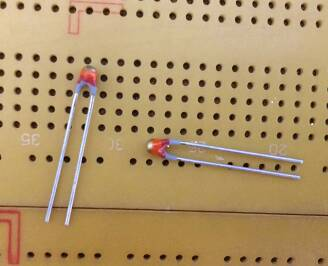
\includegraphics[width=\linewidth]{ntc.jpg}
        & Термістор, чутливий до зміни опору в залежності від температури. & Роздільна здатність: залежить від моделі, Робочий діапазон: від -50°C до +150°C, Протокол: аналоговий сигнал. \\
        \hline
        Термопара K типу
        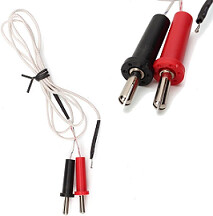
\includegraphics[width=0.7\linewidth]{thermocouple.jpg}
        & Складається з двох металевих провідників, генерує мікровольтовий сигнал при зміні температури на місці їх з'єднання. & Роздільна здатність: залежить від попарних металів -- 0.1°C, Робочий діапазон: від -270°C до +1372°C, Протокол: аналоговий сигнал. \\
        \hline
        DS18B20
        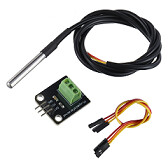
\includegraphics[width=0.77\linewidth]{ds18b20.jpg}
        & Цифровий температурний сенсор, випускається фірмою Maxim Integrated. & Роздільна здатність: 0.0625°C, Робочий діапазон: від -55°C до +125°C, Протокол: 1-Wire. \\
        \hline
        DHT11
        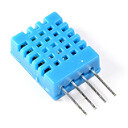
\includegraphics[width=\linewidth]{dht11.jpg}
        & Цифровий температурно-вологісний сенсор. & Роздільна здатність: 1°C, Робочий діапазон температури: від 0°C до 50°C, Протокол: спеціальний протокол на базі однопровідного інтерфейсу. \\
        \hline
        DHT22
        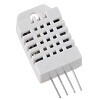
\includegraphics[width=\linewidth]{dht22.jpg}
        & Також відомий як AM2302, цифровий температурно-вологісний сенсор. & Роздільна здатність: 0.1°C, Робочий діапазон температури: від -40°C до +80°C, Протокол: спеціальний протокол на базі однопровідного інтерфейсу. \\
        \hline
        HTU21D
        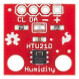
\includegraphics[width=0.6\linewidth]{htu21d1.jpg}
        & Цифровий температурно-вологісний сенсор, вироблений фірмою Measurement Specialties. & Роздільна здатність: 0.01°C, Робочий діапазон температури: від -40°C до +125°C, Протокол: I2C. \\
        \hline
    \end{tabular}
    \vspace{-3.3cm}
\end{table}

\clearpage

\section{Аналогові датчики}

\textbf{NTC терморезистор}\bigskip

Терморезистор, за своєю суттю резистор, який зроблений з напівпровідника та змінює свій опір зі зміною температури. Можна визначити два типи терморезисторів -- NTC терморезистор (термістор), який зменшує опір при нагріві (саме про них піде далі), та PTC терморезистор (позистор), який збільшує опір при нагріві. Є досить багато типів терморезисторів за формфактором, їх можна побачити на рис.~\ref{fig:thermoresistor_types}.

\begin{figure}[ht]
    \centering
    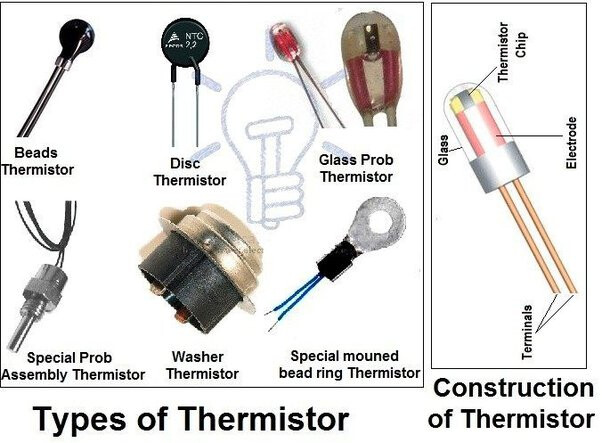
\includegraphics[width=0.7\linewidth]{thermoresistor_types.jpg}
    \caption{Різні типи терморезисторів}
    \label{fig:thermoresistor_types}
\end{figure}

На невеликому проміжку залежність опору від температури є лінійною, що дозволяє виконати апроксимацію використовуючи температурний коефіцієнт опору (TCR) для цієї області, та знаючи для якої референсної температури він відноситься (наприклад $25^\circ~C$) (рівняння \ref{eq:tcr}).

\begin{equation}
    \label{eq:tcr}
    \rho = \rho_0\left(1+\alpha\frac{t-t_0}{t_0}\right)
\end{equation}

На усьому робочому діапазоні залежність вже не лінійна, а отже розрахунки по такій формулі дадуть досить високу похибку на границях діапазону (рис.~\ref{fig:ntc_curve}).

\begin{figure}[ht]
    \centering
    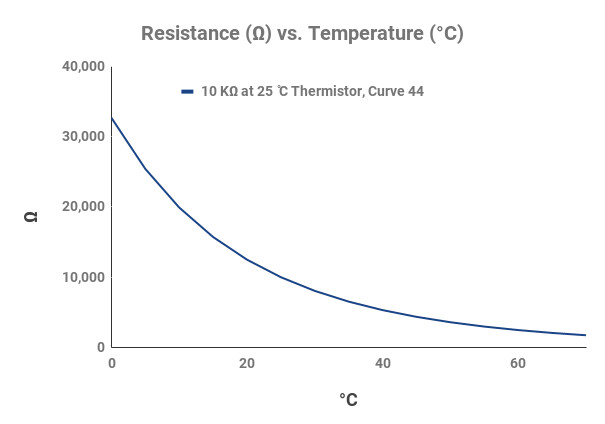
\includegraphics[width=0.9\linewidth]{ntc_curve.jpg}
    \caption{Характеристика NTC термістора}
    \label{fig:ntc_curve}
\end{figure}

Для деяких термісторів можна знайти специфікацію, у якій може бути надана таблиця залежності температури від опору з кроком 1°C або 5°C, проміжні значення можна розрахувати використовуючи лінійну інтерполяцію.

Зазвичай використовують іншу формулу для розрахунку температури з опору. Одним з параметрів, що характеризують залежність опору від температури, є коефіцієнт температурної реакції, що позначається $B$ та вимірюється у кельвінах. Цей коефіцієнт розраховується зі значень опору при двох конкретних температурах, і для багатьох термісторах може бути від 2600 до 4200K. У багатьох випадках ці температури вибирають 25°C і 100°C. Як правило, температури, використовувані при розрахунку коефіцієнта, задаються після букви, наприклад B25/100. Наступна експоненційна формула \ref{eq:ntc_beta} може бути використана для більш точних розрахунків.

\begin{equation}
    \begin{aligned}
        \text{R}_t = \text{R}_0 e^{\beta\left(\frac{1}{T}-\frac{1}{T_0}\right)}
        & \text{ , де T -- температура термістора} \\
        & \text{$T_0$ -- референсна температура} \\
        & \text{$\text{R}_0$ -- опір при референсній температурі} \\
        & \text{$\beta$ -- коефіцієнт температурної реакції}
    \end{aligned}
    \label{eq:ntc_beta}
\end{equation}

Окрім цього можна скористатися формулою Стейнхарта-Харта, яка дозволяє ще точніше розраховувати температуру, знаючи A, B, C коефіцієнти для взятого термістора (часто є у специфікації).

\begin{equation}
    \begin{aligned}
        \frac{1}{\text{T}} = A + B\ln(\text{R}) + C\left[\ln(\text{R})\right]^3
        & \text{ , де T -- температура у Кельвінах} \\
        & \text{R -- опір резистора}
    \end{aligned}
\end{equation}

\begin{figure}[ht]
    \centering
    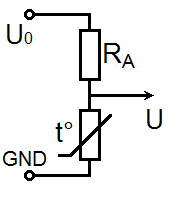
\includegraphics{ntc_connect.jpg}
    \caption{Схема підключення термістора}
    \label{fig:}
\end{figure}

Висновки по NTC термістру:

\begin{itemize}
    \item Сам по собі термістор має високу точність та малий час реакції, але без належного калібрування значення температури будуть відрізнятися на декілька градусів (особливо при зменшенні температури);
    \item Розрахунок температури можна зробити декількома способами: використовуючи рівняння, що на деяких мікропроцесорах буде сповільнювати роботу програми, або табличним способом, коли розраховуються значення температур в залежності від опору з деяким кроком, а проміжні значення отримуються за допомогою лінійної інтерполяції;
    \item Термістор вмикається в схему у верхнє або нижнє плече дільника напруги (від цього залежатиме вид характеристики). Зміна опору термістора призводить до зміни напруги дільника;
    \item Обираючи номінали дільника (резистора і термістора), слід врахувати, що струм, який протікає через термістор, спричиняє його нагрівання і, як наслідок, спотворення показань;
    \item Термістор один з найдешевших датчиків температури, що є великою перевагою.
\end{itemize}

\textbf{Термопара К-типу}\bigskip

Основною перевагою термопар є їх широкий температурний діапазон. Обмежена, по суті, абсолютним нулем (з нюансами) і температурою плавлення металів, тобто здатна робити виміри, де інші датчики просто вийдуть зі стану -- від -270 до + 1800$^\circ$C і вище.

Термопара досить цікавий датчик, адже в ній використовується інший ефект -- ефект Зеєбека, і на відміну від термістора, вона є пасивним датчиком, тобто створює дуже низьку напругу в залежності підвищення температури. Тут потрібно з'ясувати як саме вона працює.

Річ у тому, що при з'єднанні двох різнорідних сплавів провідників (наприклад Алюмель та Хромель) при їх нагріванні виникає різниці потенціалів, яка і генерує напругу. Нагрівати ми будемо так званий ``гарячий'' сплав, і зчитувати його напругу. Тут важливо зауважити, що інший -- ``холодний'' сплав, не можна нагрівати, адже саме при різних температурах виникає Електрорушійна сила, яка прямо пропорційно різниці цих температур. Термопара це відносний датчик, тому температура зовнішнього середовища до уваги не береться, важливі тільки відносини двох сплавів.

Як можна було зрозуміти, на виході (після перетворення) ми отримаємо температуру відносно холодного сплаву, а отже, щоб отримати реальну температуру на гарячому сплаві, потрібно завчасно виміряти температуру на холодному (референсному), для цього можна використати той же термістор. Цікаво, що цю проблему можна також вирішити помістивши холодний сплав у воду температури $0^\circ~C$, тоді компенсувати значення з гарячого сплаву не потрібно.

В залежності від потреб використовуються різні сплави, наприклад наша термопара К-типу використовує Алюмель (холодний) та Хромель (гарячий), і дозволяє вимірювати у досить широкому діапазоні, з кінцевими границями у $-200^\circ~C$ -- $1260^\circ~C$, таку термопару зручно використовувати для термостата у паяльні станції. Термопара Е-типу складається з Хромелю та Константану, і дозволяє вимірювати дуже низькі температури, не піддається корозії, і тому може бути використана у вологих середовищах. Також використовуються наступні сплави: E (хромель-константант), J (залізо-константант), K (хромель-алюмель), M (мідно-копель), N (ніхросил-нісил) та інші.

Як було сказано вище, термопара генерує низьку напругу, К-типу -- 0.4мВ/$^\circ$C, АЦП з роздільною здатністю 10 бітів не здатен зчитати таку напругу, тому її потрібно спочатку підсилити за допомогою неінвертуючого підсилювача, про це більш детально у практичній частині.

Для перетворення значення з підсиленого виходу термопари у температуру скористуємося наступною формулою \ref{eq:thermocouple}.

\begin{equation}
    \label{eq:thermocouple}
    \begin{aligned}
        T = \frac{V}{Ga} + T_{\text{ref.}}
        & \text{ , де V -- підсилений сигнал} \\
        & \text{G -- коефіцієнт підсилення} \\
        & \text{$\alpha$ -- коефіцієнт Зеєбека, табличне значення} \\
        & \text{$T_{\text{ref.}}$ -- температура холодного сплаву}
    \end{aligned}
\end{equation}

\begin{figure}[ht]
    \centering
    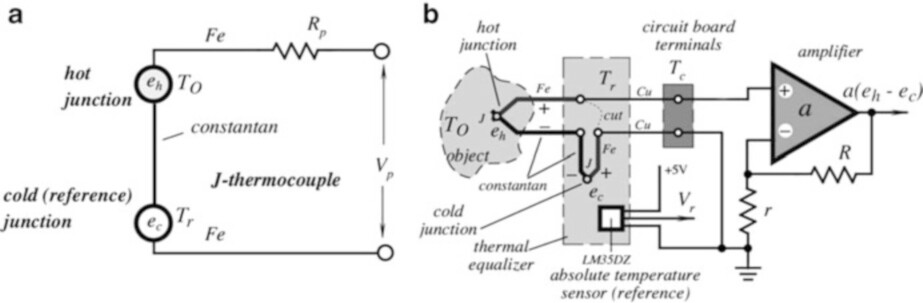
\includegraphics[width=\linewidth]{thermocouple_usage.jpg}
    \caption{Приклад використання термопари}
    \label{fig:thermocouple_usage}
\end{figure}
%\FloatBarrier

Висновки по термопарі К-типу:

\begin{itemize}
    \item Більше ніяких складних формул, у термопарі К-типу ми маємо лінійну залежність 0.4мВ/$^\circ$C вище нуля, все що потрібно це підсилити цю напругу та скористатися простою формулою;
    \item Термопара має нижчу швидкість реакції, а той же час здатна вимірювати високі температури;
    \item Має непогану точність, але її складно досягти, без ізоляцій і фільтрів на входах та виходах. Термопара К-типу має майже лінійну залежність, тому калібровка не є складно. Ці нюанси не такі вже і важливі, адже термопарою вимірюють високі температури, де похибка у декілька градусів не страшна.\\
\end{itemize}


\section{Цифрові датчики}

З попередньої частини про аналогові датчики можна було з'ясувати, що працювати з ними важко, потрібно використовувати складні формули для перетворення напруги в одиниці вимірювання температури, часто потрібно використовувати фільтри сигналу, щоб запобігти значного спотворення сигналу доки він дійде до АЦП. У випадку с термопарою ситуація виходить ще складніша, адже окрім фільтрації потрібно ще знати температуру холодного сплаву, і додавати її або програмним способом, або просто у схемі з'єднавши послідовно термопару та схему компенсації, яка повинна генерувати напругу з тим же шагом (0.4мВ/$^\circ$C) (рис.~\ref{fig:thermocuple_cold_junction_compensation}).
\enlargethispage{\baselineskip}

\begin{figure}[ht]
    \centering
    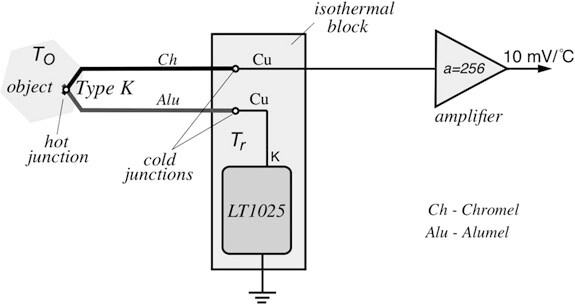
\includegraphics[width=0.8\linewidth]{thermocouple_cj_compensation.jpg}
    \caption{Додавання сигналів з термопари та компенсатора холодного сплаву}
    \label{fig:thermocuple_cold_junction_compensation}
\end{figure}

Ці недоліки, коли потрібна максимальна простота з боку схемотехнічної реалізації та надійність, яку дає виробник, приводить нас до цифрових датчиків. Вони містять у собі АЦП, інтегральну мікросхему, фільтри, і на виході генерують дискретний сигнал, який передають по спеціальних шинах даних стійких до завад (принаймні, на малій відстані). Існує безліч цифрових датчиків, про деякі з них піде річ далі.\\

\textbf{DS18B20}\bigskip

Один з найпопулярніших цифрових датчиків температури, який виробляється фірмою Maxim Integrated. Передача даних відбувається за допомогою пропрієтарної дуплексної шини даних 1-Wire, яка використовує одну лінію для взаємодії з підключеними девайсами. На шину можна під'єднати безліч датчиків, адже кожен з них має свій унікальний номер. Датчик потребує живлення 5В, яке також може подаватися через шину дану (паразитне живлення). Шину даних потрібно підтягнути до живлення резистором ~5 кОм. На рис.\ref{fig:ds18b20_scheme} зображена внутрішня реалізація датчику.

\begin{figure}[ht]
    \centering
    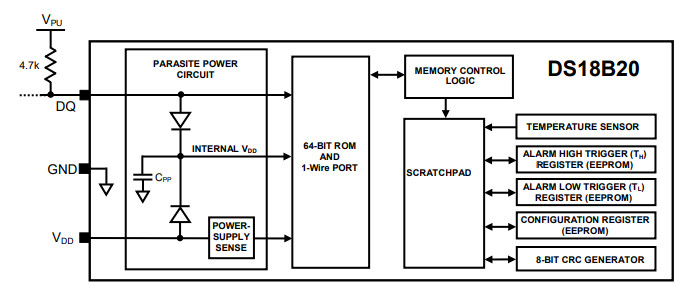
\includegraphics[width=\linewidth]{ds18b20_scheme.jpg}
    \caption{Внутрішня структура DS18B20}
    \label{fig:ds18b20_scheme}
\end{figure}

Датчик здатен вимірювати температуру у діапазоні від -55$^\circ$C до 125$^\circ$C з точністю 0.5$^\circ$C. Роздільну здатність можна також налаштувати від 9 до 12 бітів (за замовчуванням 12), тобто, наприклад 11 бітів відповідають {$\frac{125-(-55)}{2^{11}}~\approx~0.09^\circ$C} ``чутливості''. За специфікацією маємо наступні калібровані значення: 0.5$^\circ$C, 0.25$^\circ$C, 0.125$^\circ$C, 0.0625$^\circ$C. Щобільше обрана розрядність, то повільніше буде вимірювати температуру датчик: 93.75 мс, 187.5 мс, 375 мс, 750 мс.

Після посилання команди на вимір температури, в залежності від розрядності, вимір займе вищевказаний час. Датчик зберігає температуру у 16 бітний регістр, який після вимірювання потрібно зчитувати.

\begin{figure}[ht]
    \centering
    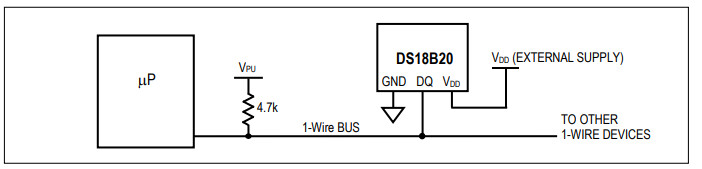
\includegraphics[width=\linewidth]{ds18b20_connect.jpg}
    \caption{Приклад підключення датчика}
    \label{fig:}
\end{figure}

В цілому цей датчик має низьку ціну, дозволяє за допомогою інтерфейсу 1-Wire організувати мережу датчиків, що охоплюють ту чи іншу область. Наприклад, декілька датчиків можна встановити у теплиці та контролювати температуру. Взагалі, саме такі проєкти є головними споживачами цього датчика.\\

\textbf{DHT11}\bigskip

На відміну від попереднього датчика цей є більше простим, але окрім темеператури дозволяє вимірювати вологість. Передача даних відбувається за допомогою однопровідної шини даних використовуючи простий протокол для комунікації. Не підтримує під'єднання декількох датчиків на одну шину.

Може працювати від напруги 3.3 до 5 В. Шина даних підтягується до живлення резистором ~5 кОм. Для вимірювання температури використовує термістор, а коефіцієнти калібрування записані на read-only OTP пам'яті. Точність DHT11 зазвичай становить +/-2$^\circ$C для температури та +/- 5\% для вологості. Роздільна здатність -- 1$^\circ$C. Резистивний елемент, вбудований у датчик, реагує на зміни вологості.

У цьому датчику не має вбудованої пам'яті для збереження результатів вимірювань, а час вимірювання становить 2 секунди, а у найгірших випадках до 30 секунд.

\begin{figure}[ht]
    \centering
    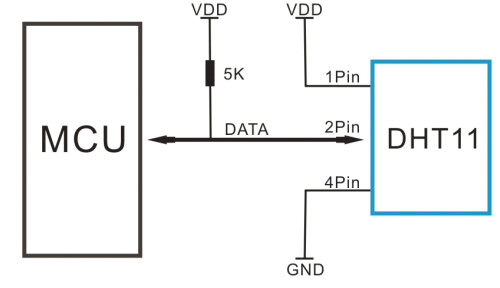
\includegraphics[width=0.6\linewidth]{dht11_connect.jpg}
    \caption{Приклад підключення датчика}
    \label{fig:}
\end{figure}

Взагалі, датчик можна вважати невдалим, і його використання навіть у проєктах теплиці є великим питанням. Має низьку ціну, але водночас усі його характеристики є поганими, порівнюючи з іншими датчиками. Не рекомендується для використання.\\

\textbf{DHT22}\bigskip

Датчик DHT22, також відомий як AM2302, є вдосконаленою версією DHT11, надаючи покращену точність та ряд інших характеристик для вимірювання температури та вологості. Для передачі даних DHT22 використовує простий цифровий інтерфейс, але у порівнянні з DHT11, має меншу частоту оновлення даних, що робить його більш стійким до зовнішніх перешкод.

Побудований також на базі термістора, використовує конденсаторні елементи для вимірювання вологості. Зміна вологості впливає на діелектричні властивості конденсаторів, що визначається мікроконтролером для визначення вологості повітря. На відміну від DHT11 використовує шкалу компенсації температурних змін, що дозволяє коригувати вимірювання вологості в залежності від змін температури, щоб забезпечити точніші результати в різних умовах. Також має певну стійкість до зовнішніх впливів, таких як конденсація водяної пари.

DHT22 вимірює температуру від -40 до 80$^\circ$C та вологість від 0\% до 100\%. Точність DHT22 зазвичай становить +/- 0.5$^\circ$C для температури та +/- 2\% для вологості. Роздільна здатність - 0.1$^\circ$C.

Таким чином, DHT22 є більш розвиненою версією DHT11. Він має вищу точність вимірювань, а також можливості компенсації температурних змін.\\

\textbf{HTU21D}\bigskip

Датчик HTU21D1 є цифровим датчиком вологості та температури, розробленим компанією Measurement Specialties. Він відзначається високою точністю вимірювань та компактним дизайном.

Для передачі сигналу у цифровому сигналі використовує шину I²C, що дозволяє дуже просто його підключати та використовувати багато пристроїв на єдиній шині. Датчик має низьке енергоспоживання (максимальна напруга -- 3.8В, струм у стані спокою -- 0.02 мкА, у стані вимірювання -- до 500 мкА) та є більш чутливим до змін температури. Має високу точність вимірювань. Точність для вологості може сягати до +/- 2\%, а для температури -- до +/- 0.3°C. Не потребує калібрації, адже кожен датчик індивідуально калібрується і тестується. Номер партії друкується на датчику, а його власний ідентифікатор зберігається на мікросхемі, який можна зчитати за допомогою команди. Роздільна здатність може бути змінена за допомогою команди (11 -- 14 бітів для температури та 8 -- 12 для вологості). Тобто роздільна здатність при максимальній розрядності 12 бітів отримаємо роздільну здатність ~ 0.01$^\circ$C.

Датчик забезпечує вимірювання вологості в діапазоні від 0\% до 100\% та температури від -40°C до 125°C. Датчик має вбудований нагрівний елемент, який здатен підвищити температуру на 1.5$^\circ$C. Як і попередній датчик здатен компенсувати температуру при вимірюванні вологості від 0 до 80$^\circ$C.

На відміну від усіх попередніх цифрових датчиків, час виміру температури не перевищує 50 мс при максимальній роздільній здатності.

Специфікація надає формули для виміру приблизної точки роси використовуючи зчитану температуру та вологість (формули \ref{eq:dew_point1}-\ref{eq:dew_point2})

\begin{equation}
    \begin{aligned}
        PP_{Tamb} = 10^{\left[A-\frac{B}{\left(T_{Amb}+C\right)}\right]}
        & \text{ , де T -- виміряна температура} \\
        & \text{A, B, C -- константи 8.1332, 1762.39, 235.66}
    \end{aligned}
    \label{eq:dew_point1}
\end{equation}

\begin{equation}
    \begin{aligned}
        T_d = -\left[\frac{B}{\log_{10} \left(RH_{amb}\cdot\frac{PP_{Tamb}}{100}\right)-A}+C\right]
        & \text{ , де $T_d$ -- точка роси} \\
        & PP_{Tamb} \text{ -- парціальний тиск} \\
        & RH_{amb} \text{ -- вологість повітря}
    \end{aligned}
    \label{eq:dew_point2}
\end{equation}




\chapter*{Висновки до Розділу 1}
\addcontentsline{toc}{chapter}{Висновки до Розділу 1}

У першому розділі курсової роботи були розглянуті загальні характеристики датчиків, обґрунтований вибір температурних датчиків для проведення експерименту, а також розглянуті обрані датчики з точки зору їх застосування, внутрішньої реалізації та принципу їх роботи. Особлива увага була приділена саме до останнього пункту -- принципу роботи аналогових та цифрових датчиків. Так, було визначено, що аналогові датчики у разі ретельного калібрування дають точні результати вимірювань, та окрім цього дають по суті необмежену роздільну здатність (обмежена тільки АЦП мікроконтролера) та швидкість вимірювання. 

По-перше, був розглянутий термістор, і з'ясовано, що він не потребує складного підключення, але потребує калібрації, або за допомогою таблиці, або використовуючи коефіцієнти для розрахунків. Отже, маючи невідомий NTC термістор, можна лише приблизно його відкалібрувати, наприклад зробивши виміри температури на крайніх точках, та по середині діапазону, так ми отримаємо деяке покращення точності.

По-друге, була розглянута термопара, яка у теорії ідеальний інструмент для вимірювання високих та низьких температур, але потребує значно складнішої схеми для фільтрування та підсилення сигналу. Окрім цього, потрібен зовнішній датчик, який би виміряв температури холодного сплаву.

Далі були розглянуто декілька цифрових датчиків, які значно простіші у використанні, не потребують складних формул та схем. Це компенсується нижчою швидкістю роботи (аж до 2 секунд), та обмеженою роздільною здатністю. При цьому, усі коефіцієнти для калібрування збережені у самому датчику і не потребують зміни зі зміною середовища.

У наступному розділі буде зібрано макет для тестування датчиків, та виводу їх вимірювань на LCD дисплей.

\chapter{Розробка макету для тестування датчиків}
\thispagestyle{headings}

\section{Підключення датчиків у Proteus}

\textbf{NTC}\bigskip

Схему макету будемо збирати у Proteus, він дозволяє повноцінно симулювати прості схеми, великим мінусом є той факт, що схема у Proteus працює без похибок та завад, при збірці схеми на макетній платі результати з датчиків будуть дещо відрізнятися.

Arduino не може виміряти опір резистора, тому потрібно зібрати класичну схему з відомим резистором, так невідомим (наш NTC термістор). Опір відомого повинен буде якнайближче до опору невідомого, у нашому випадку NTC термістор має опір 10 кОм, що відповідає 25$^\circ$C. У якості живлення будемо використовувати 3.3 В, адже воно має менше шумів, на реальному макеті також будемо використовувати його як референсне (AREF).

На рис.~\ref{fig:ntc_proteus} можна побачити схему підключення термістора, опір відомого резистора був виміряний на реальній схемі мультиметром, щоб досягти більш точних результатів. Під'єднаємо термістор на A0 пін.

\begin{figure}[ht]
    \centering
    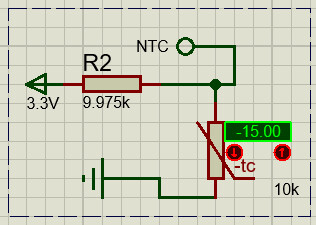
\includegraphics{ntc_proteus.jpg}
    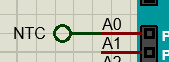
\includegraphics{ntc_proteus2.jpg}
    \caption{Підключення NTC термістора}
    \label{fig:ntc_proteus}
\end{figure}

Щодо роботи з NTC термістором був написаний окремий клас (ліст.~\ref{lst:ntc}) який є спадком базового класу Sensor (ліст.~\ref{lst:sensor_base}), який зчитує напругу та знаючи опір відомого резистора, підраховує опір термістора. Далі за формулою \ref{eq:ntc_beta} отримаємо температуру у градусах Цельсія.\\

\textbf{Термопара К-типу}\bigskip

Як було сказано раніше, термопара дещо відрізняється від підключення інших датчиків, а саме вона є пасивним датчиком та генерує дуже малу напругу при зміні температури (~ 41 мкВ/$^\circ$C), тому потрібно підсилити сигнал за допомогою неінвертуючого операційного підсилювача.

За допомогою потенціометра було підібрано резистор для на зворотного зв'язку (чим менше опір -- тим більше коефіцієнт підсилення). Для підсилення сигналу було обрано подвійний операційний підсилювач LM358N.

\begin{figure}[ht]
    \centering
    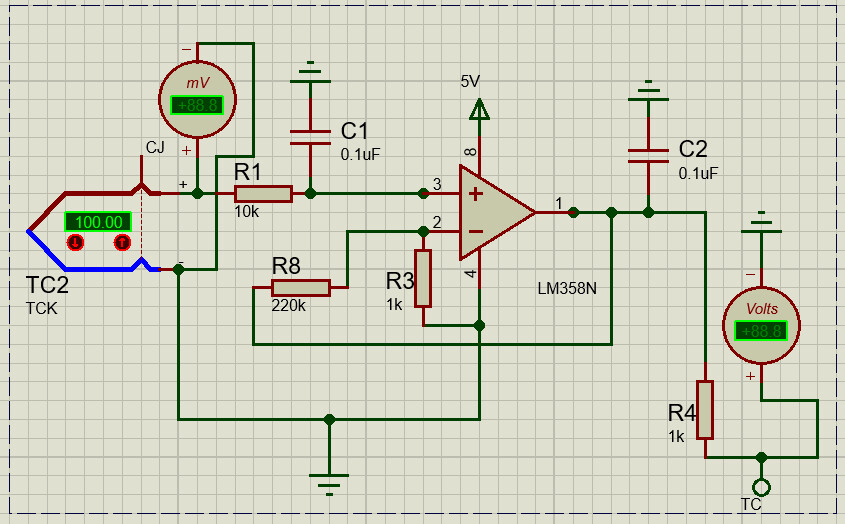
\includegraphics[width=0.8\linewidth]{thermocouple_proteus.jpg}
    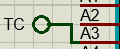
\includegraphics{thermocouple_proteus2.jpg}
    \caption{Підключення термопари К-типу}
    \label{fig:thermocouple_proteus}
\end{figure}

Взагалі це не найкращий вибір мікросхеми для підсилення напруги термопари, адже шумить та сильніше підсилює сигналу відносно до коефіцієнта підсилення. Наприклад можна було встановити спеціалізовану мікросхему AD8495 для термопар К-типу, яка не тільки підсилює сигнал, а ще й виконує компенсацію холодного сплаву за допомогою вбудованого датчика температури. Іншим вибором може бути готова мікросхема від Adafruit -- MAX31865, з якої можна зчитувати конвертовану температуру за допомогою інтерфейсу SPI.

Як було зазначено у формулі \ref{eq:thermocouple}. для того, щоб визначити температуру потрібно знати коефіцієнт підсилювання -- $G = 1+\frac{R_f}{R_{in}} = 1+\frac{220000}{1000} = 221$, але перевіривши експериментальним шляхом було визначено, що це значення не відповідає реальному. Складемо рівняння з невідомим коефіцієнтом підсилення, інші дані відомі після вимірювання. Підставимо ці значення, та знайдемо коефіцієнт підсилення (\ref{eq:tc_gain}). Як можна побачити коефіцієнт значно відрізняється, що могло значно погіршити результати вимірювань. Окрім цього, як було визначено пізніше, операційний підсилювач, також шумить, тобто коли на термопарі мультиметр показує 0 мкВ, на виході підсилювача -- ~5 мВ. АЦП входи Arduino також шумлять, додаючи ~20 мВ. Отже, значення можна скоригувати програмно, віднявши максимум 0.03 В.

\begin{equation}
    \begin{aligned}
        \frac{V}{Ga} + T_{ref} &= T \\
        \frac{0.452}{G\cdot0.000041} + 22.8 &= 57 \\
        G~&\approx~322.35
    \end{aligned}
    \label{eq:tc_gain}
\end{equation}

Табличне значення коефіцієнта Зеєбека -- для термопари К-типу ~41 мкВ/$^\circ$C, температура холодного сплаву -- будемо вимірювати за допомогою NTC термістора та сигнал на виході підсилювача.

Для роботи з термопарою було написано відповідний клас (ліст.~\ref{lst:tc_sensor}), що є нащадком класу Sensor (див. ліст.~\ref{lst:sensor_base}).\\ 

\textbf{DS18B20}\bigskip

На відміну від аналогових датчиків, при підключенні цифрових на повинно виникати складнощів. Вихід даних зазвичай підтягують на живлення використовуючи резистор на ~5 кОм, на це особливо потрібно звертати увагу, коли датчик знаходиться за кілька метрів від мікроконтролера.

На рис.~\ref{fig:ds18b20_proteus} можна побачити підключення цього датчику. Датчик працює по протоколу 1-Wire, для економа часу було використану бібліотеку microDS18B20 для зчитування температури з датчика. Додатковий клас для роботи з цим датчиком та конфігурація у ліст.~\ref{lst:ds18_sensor}.

\begin{figure}[H]
    \centering
    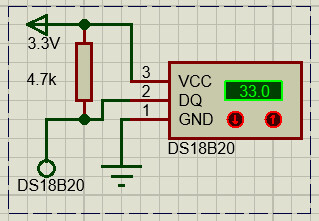
\includegraphics{ds18b20_proteus.jpg}
    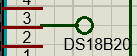
\includegraphics{ds18b20_proteus2.jpg}
    \caption{Підключення датчику DS18B20}
    \label{fig:ds18b20_proteus}
\end{figure}

\textbf{DHT11 та DHT22}\bigskip

Ці датчики також були підключені до живлення 3.3 В, а опір резистора для підтягування був обраний згідно зі специфікацією. На рис.~\ref{fig:dht_proteus} можна побачити підключення цього датчику. Для роботи з датчиками була використана бібліотека ``DHT sensor library'' від Adafruit. Робота з ним також була винесена в окремий клас (ліст.~\ref{lst:dht_sensor}).

\begin{figure}[ht]
    \centering
    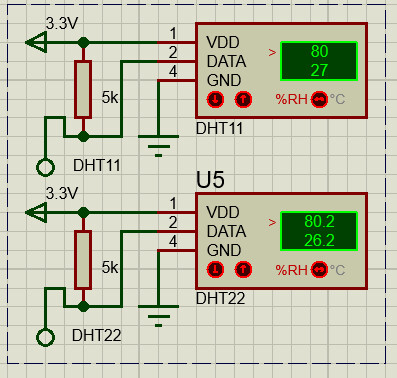
\includegraphics{dht_proteus.jpg}
    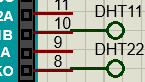
\includegraphics{dht_proteus2.jpg}
    \caption{Підключення датчику DHT11/DHT22}
    \label{fig:dht_proteus}
\end{figure}
\clearpage
\textbf{HTU21D}\bigskip

У моделі Proteus до датчика не можна під'єднати зовнішнє живлення, на макетній платі також будемо використовувати живлення 3.3 В. Цей датчик використовує комунікацію за допомогою I2C шини, беручи до уваги те, що у кожного датчика свій унікальний номер, на цю шину у теорії можна підключити безліч таких датчиків, і окрім цього LCD дисплей, який теж під'єднаємо через I2C шину. На рис.~\ref{fig:htu21_proteus} можна побачити цей датчик з винесеними пінами. Для роботи з датчиком була використана бібліотека HTU2xD\_SHT2x\_Si70xx. Клас для роботи з цим датчиком -- ліст.~\ref{lst:htu21_sensor}.

\begin{figure}[ht]
    \centering
    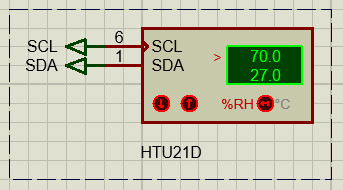
\includegraphics[scale=0.65]{htu21_proteus.jpg}
    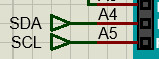
\includegraphics[scale=0.65]{htu21_proteus2.jpg}
    \caption{Підключення датчику HTU21D}
    \label{fig:htu21_proteus}
\end{figure}

\section{Перевірка роботи моделі у Proteus та на макетній платі}

Зібравши усе до купи та під'єднавши LCD дисплей через I2C модуль була написана програмна частина (ліст.~\ref{lst:program}). Очевидно, що інформація відразу з усіх датчиків не поміститься на екран, тому будемо використовувати кнопку для переходу до наступного датчика, яку під'єднаємо за допомогою внутрішньої підтяжки Arduino -- INPUT\_PULLUP.

На рис.~\ref{fig:scheme_test} можна побачити перевірку роботи схеми та програми. Перемикання між екранами здійснюється за допомогою кнопки: один натиск -- наступний датчик, два -- попередній. Робота з кнопкою винесена в окремий клас Button (ліст.~\ref{lst:button}). Використовується Timer (ліст.~\ref{lst:timer}) для запобігання блокування головного циклу програми.

Перевірку зчитування інформації з інших датчиків можна побачити на рис.~\ref{fig:tc_test} -- \ref{fig:dht11_test}.

\begin{figure}[ht]
    \centering
    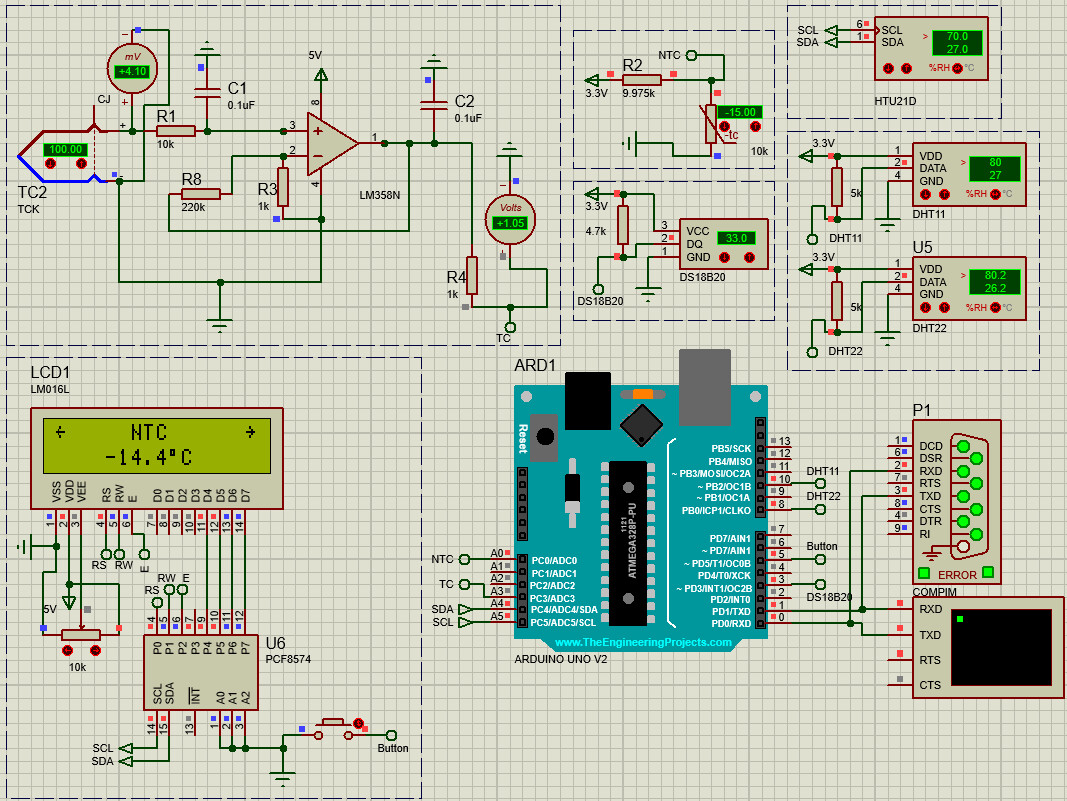
\includegraphics[width=\linewidth]{scheme_test.jpg}
    \caption{}
    \label{fig:scheme_test}
\end{figure}

На макетній платі також була зібрана демонстраційна схема (рис.~\ref{fig:scheme_real}).

\begin{figure}[!hb]
    \centering
    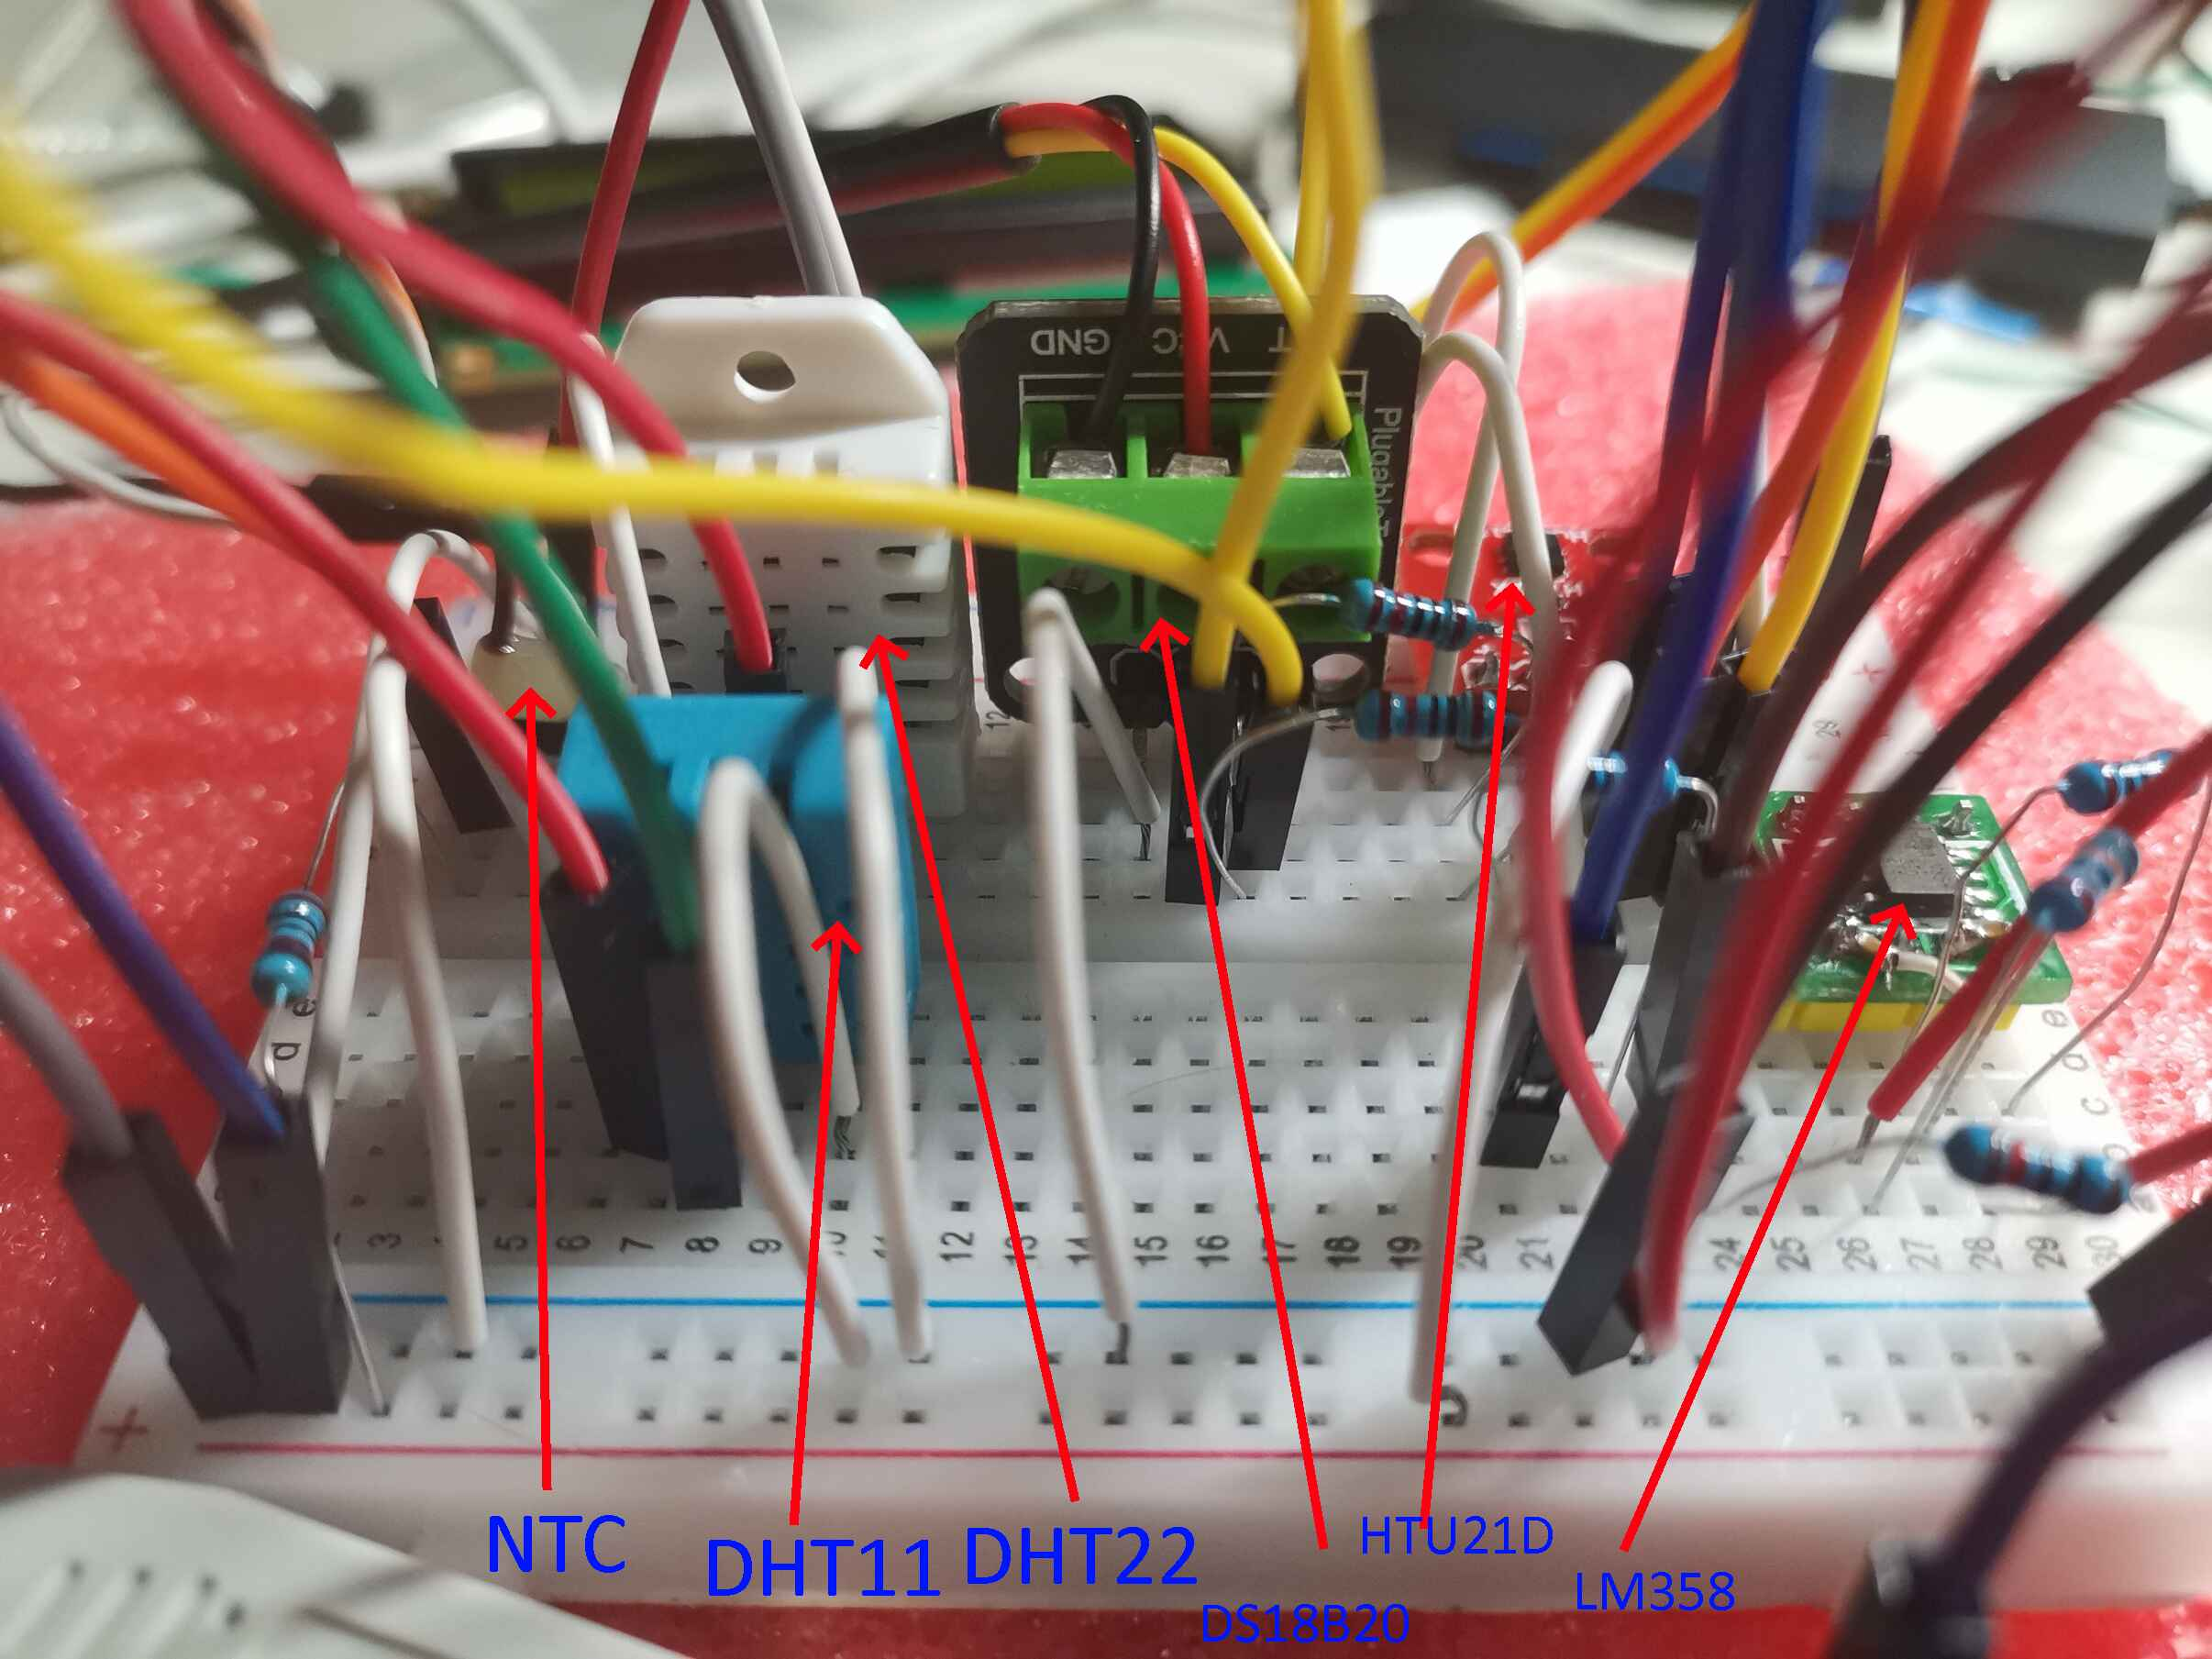
\includegraphics[width=0.75\linewidth]{scheme_real.jpg}
    \caption{Датчики на макетній платі}
    \label{fig:scheme_real}
\end{figure}

Перевірку роботи схеми можна побачити на рис.~\ref{fig:tc_test2} -- \ref{fig:ds18_test2}.\\

\section{Тестування датчиків}

Для перевірки роботи датчиків було побудовано декілька графіків. Як можна побачити на рис.~\ref{fig:plot_normal}, усі датчики видають різні значення при кімнатній температурі, підвищуючи чи знижуючи температуру, але це зовсім не означає, що тільки єдиний датчик, наприклад HTU21D показує правильну температуру. По-перше, сама температура може відрізнятися навіть на відстані декількох сантиметрів, по-друге, в кожного з датчиків у специфікації заявлена можлива похибка.

\begin{figure}[ht]
    \centering
    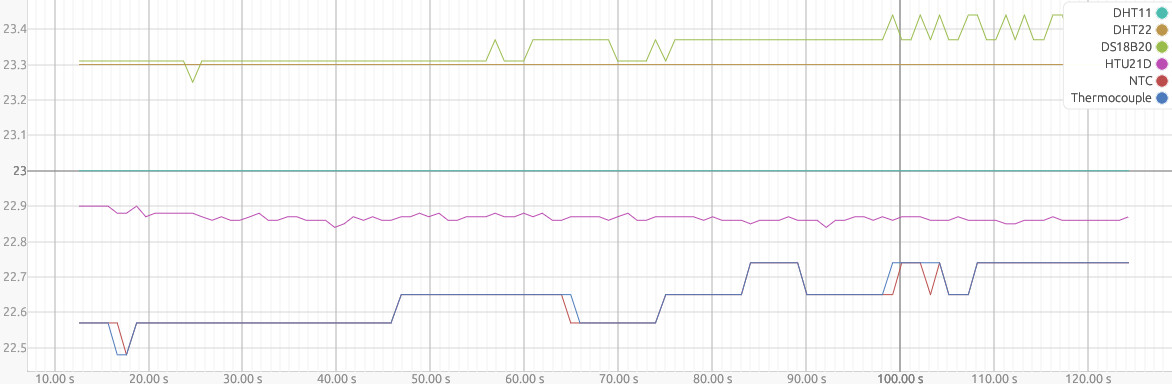
\includegraphics[width=\linewidth]{plot_normal.jpg}
    \caption{Показання датчиків при кімнатній температурі}
    \label{fig:plot_normal}
\end{figure}

У наступному експерименті на відстані ~10 см макетна плата (усі датчики були якнайближче встановлені один до одного) була обдута феном. Як можна побачити на рис.~\ref{fig:plot_hot} цифрові датчики відреагували найповільніше, а у датчиках DHT11/DHT22 спочатку нагрівся корпус, який поступово передав температуру сенсору. DS18B20 показав дещо кращий результат, адже його корпус -- сталь, яка має вищу теплопровідність. HTU21D1 показав кращий результат при спаді температури. Лідером по часу реакції стала термопара, адже її точка з'єднання гарячого та холодного сплаву менша, навіть, за термістор і також зроблена з металу.

\begin{figure}[H]
    \centering
    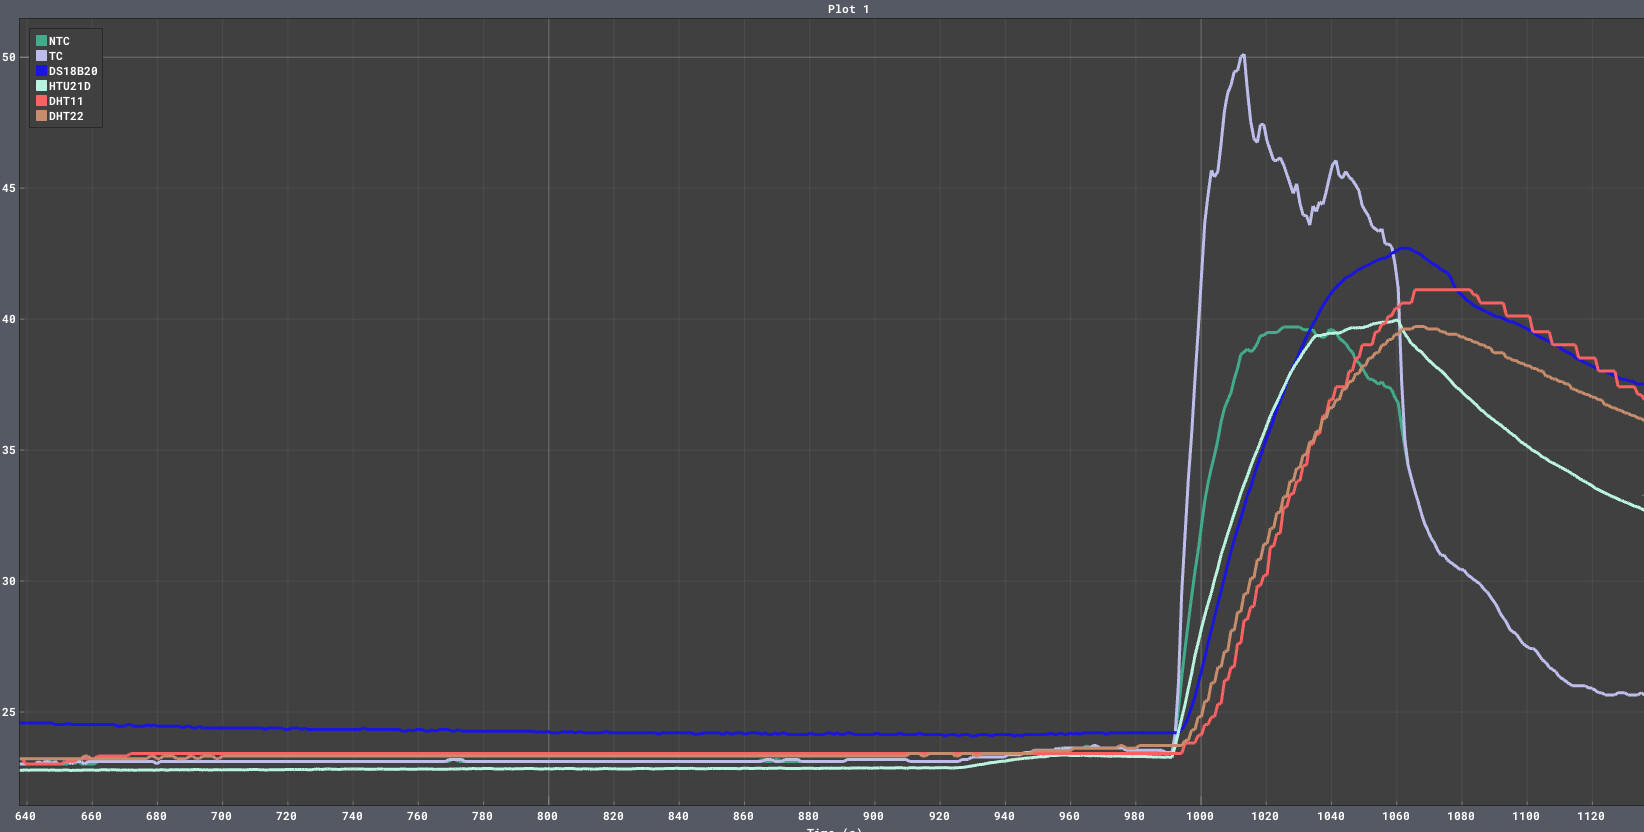
\includegraphics[width=\linewidth]{plot_hot.jpg}
    \caption{Показання датчиків при обдуванні феном}
    \label{fig:plot_hot}
\end{figure}

У теоретичній частині було заявлено, що термопара здатна вимірювати високі температури, перевіримо це за допомогою фену для пайки. Налаштуємо на ньому температуру 350$^\circ$C (рис.~\ref{fig:station}), хоча й і є великі сумніви щодо вбудованого у паяльну станцію датчику. Окрім цього, гаряче повітря буде не рівномірним, тому буде складно досягти саме 350$^\circ$C на термопарі. На термопарі під час нагріву вдалося отримати температуру 348$^\circ$C (рис.~\ref{fig:tc_test3}). На рис.~\ref{fig:plot_station} можна побачити графік нагрітої термопари.

\begin{figure}[ht]
    \centering
    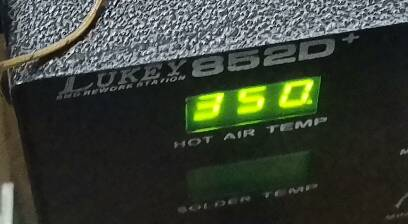
\includegraphics[scale=0.6]{station.jpg}
    \caption{Температура на паяльній станції}
    \label{fig:station}
\end{figure}

\begin{figure}[ht]
    \centering
    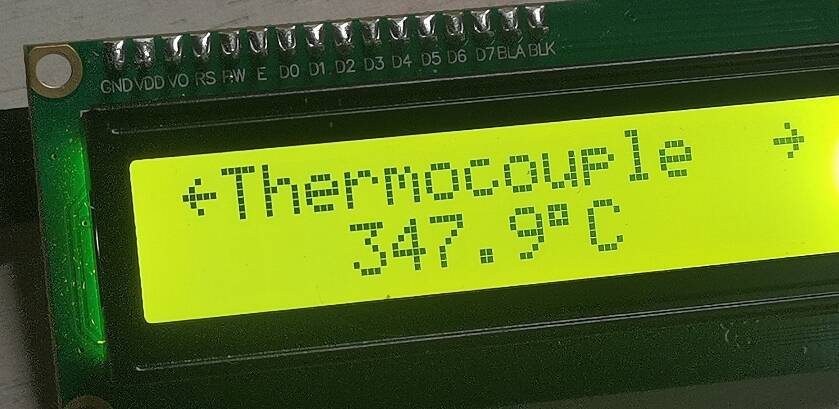
\includegraphics[width=0.4\linewidth]{tc_test3.jpg}
    \caption{Температура на термопарі}
    \label{fig:tc_test3}
    \vspace*{-3em}
\end{figure}

\begin{figure}[ht]
    \centering
    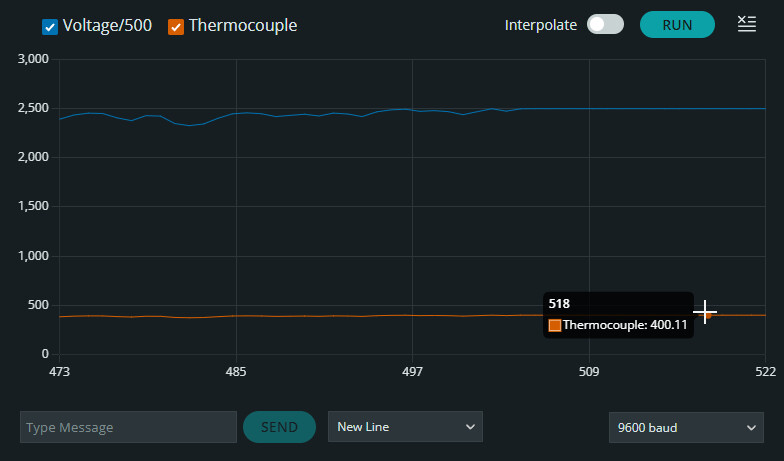
\includegraphics[width=\linewidth]{thermocouple_temp.jpg}
    \caption{Графік нагрітої термопари}
    \label{fig:plot_station}
\end{figure}


\chapterhere*{Висновки до Розділу 2}
\addcontentsline{toc}{chapter}{Висновки до Розділу 2}

У другому розділі курсової роботи на основі теоретичного матеріалу по аналоговим та цифровим датчикам була розроблена схема у Proteus та макет для тестування датчиків та перевірки їх характеристик. Була написана програмна частина, яка виводить дані з датчиків на LCD дисплей та дозволяє перемикатися між датчиками за допомогою кнопки. Додатково був зроблений вивід графіків з датчиків на екран, для візуалізації результатів. По графіках було визначено, що датчики працюють із заявленими характеристиками, такими як: час реакції, точність вимірювання. Так, датчиком з найменшим часом реакції стала термопара, а найповільнішим -- DHT11. У цілому можна сказати, що DS18B20 завищує температуру, а термістор навпаки -- занижує. Термопару, довелося додатково калібрувати, щоб знизити шуми на виході підсилювача та вході АЦП.

\chapter*{Висновки}
\addcontentsline{toc}{chapter}{Висновки}

Курсова робота полягала у порівняння аналогових та цифрових датчиків температури, та дозволила детально вивчити та порівняти різні типи температурних датчиків. У першому розділі були розглянуті загальні характеристики датчиків, здійснений вибір для експерименту та детальний аналіз обраних аналогових та цифрових датчиків.

Висновки з аналогових датчиків показали, що термістор, хоча й простий у підключенні, вимагає деякого калібрування для досягнення точності. Термопара, хоча ідеальна для екстремальних температур, потребує складнішої схеми та калібрування для отримання стабільних вимірювань. 

З іншого боку, цифрові датчики, представилися простими у використанні та не вимагають складних калібрувань. Однак, їхні обмеження в роздільній здатності та швидкості роботи були виявлені в результаті експерименту.

У другому розділі була розроблена схема та макет для тестування датчиків. Експеримент підтвердив, що датчики працюють із визначеними характеристиками.

У цілому, курсова робота дала змогу більше детально зрозуміти методи роботи з датчиками, а також той факт, що проводити тестування датчиків досить складно не в лабораторних умовах, адже точну та стійку температуру для калібрації отримати надзвичайно важко.

\printbibliography[heading=bibintoc, title=Список використанних джерел]

\begin{appendices}
    \AddAssociatedCounters{chapter}{appendixchapters}

\chapter{Код програми}
\thispagestyle{headings}

\begin{lstlisting}[style=cpp-small, caption=Базовий клас температурного датчика, label=lst:sensor_base]
enum class SensorType {
    kNTC,
    kDS18,
    kDHT11,
    kDHT22,
    kHTU21,
    kThermocouple
};

class Sensor {
    public:
    Sensor(const char *label, uint16_t interval): label_(label), interval_(interval) {}
    ~Sensor() {};
    const char* getLabel() const { return label_; };
    uint16_t getInterval() const { return interval_; };
    void getCachedInfo(float *temp, float *humidity) {
        *temp = temp_;
        *humidity = humidity_;
    }

    virtual bool begin() { return true; };
    virtual bool requestTemp() { return true; };
    virtual SensorType getType() const = 0;
    virtual void getInfo(float *temp, float *humidity = nullptr) = 0;

    protected:
    const char *label_;
    uint16_t interval_;
    float temp_ = INFINITY;
    float humidity_ = -1;

    protected:
    inline void setCachedInfo(float temp, float humidity = -1) {
        temp_ = temp;
        humidity_ = humidity;
    }
    inline void setHumidity(float *humidity, float humidity_ = -1) {
        if (humidity == nullptr) return;
        *humidity = humidity_;
    }
};

template<SensorType Type, class T = void*>
class TypedSensor: public Sensor {
    public:
    TypedSensor(T sensor, const char *label, uint16_t interval): Sensor(label, interval), sensor_(sensor) {}
    TypedSensor(const char *label, uint16_t interval): Sensor(label, interval) {}

    inline SensorType getType() const override final {
        return Type;
    }

    protected:
    T sensor_;
};
\end{lstlisting}

\begin{lstlisting}[style=cpp-small, caption=Клас для роботи з термістром, label=lst:ntc]
template<uint8_t Pin, uint16_t BCoeff, uint8_t NominalTemp = 25>
class NTC {
    public:
    NTC(uint32_t series_res, uint32_t nominal_res = 10000) {
        pinMode(Pin, INPUT);
        series_nominal_ratio_ = (float)series_res/nominal_res;
    }

    static float analogToCelsius(uint16_t analog, float series_nominal_ratio) {
        float temp = series_nominal_ratio * (float)analog / (1023.f - analog);

        temp = log(temp) / (float)BCoeff;
        temp += 1.f /((float)NominalTemp + 273.15);
        return (1.f / temp) - 273.15;
    }

    float getTemperature() {
        uint16_t analog = analogRead(Pin);
        return analogToCelsius(analog, series_nominal_ratio_);
    }

    float getTemperatureAverage(uint8_t samples = 64) {
        uint16_t sum = 0;
        for (uint8_t i = 0; i < samples; ++i) {
            sum += analogRead(Pin);
        }
        return analogToCelsius((float)sum / samples, series_nominal_ratio_);
    }

    private:
    float series_nominal_ratio_ = 1.0;
};
\end{lstlisting}

\begin{lstlisting}[style=cpp-small, caption=Клас-спадок базового класу Sensor для роботи з NTC термістром, label=lst:ntc_sensor]
#include "NTCSensor.h"
#include "Sensor.h"

template<SensorType Type, class T>
class NTCSensor: public TypedSensor<Type, T> {
    public:
    NTCSensor(T sensor, const char *label, uint16_t interval): TypedSensor<Type, T>(sensor, label, interval) {}

    void getInfo(float *temp, float *humidity = nullptr) override {
        *temp = this->sensor_->getTemperatureAverage();
        this->setHumidity(humidity);
        this->setCachedInfo(*temp);
    }
};

#define NTC_PIN A0
#define NTC_R 9975
#define NTC_R1 10000
#define NTC_T 25
#define NTC_B 3950

#define NTC_INTERVAL 500
const char ntc_label[] PROGMEM = "NTC";

using NTCConf = NTC<NTC_PIN, NTC_B, NTC_T>;
NTCConf ntc(NTC_R1, NTC_R);
NTCSensor<SensorType::kNTC, NTCConf*> ntc_sensor(&ntc, ntc_label, NTC_INTERVAL);
\end{lstlisting}

\begin{lstlisting}[style=cpp-small, caption=Клас-спадок базового класу Sensor для роботи з термопарою К-типу, label=lst:tc_sensor]
#include "NTC.h"
#include "Sensor.h"

template<SensorType Type, class T, uint8_t Pin, uint16_t OpAmpGain>
class ThermocoupleSensor: public TypedSensor<Type, T> {
    public:
    ThermocoupleSensor(T sensor, const char *label, uint16_t interval, float seebeck_coeff = 0.0000414): TypedSensor<Type, T>(sensor, label, interval) {
        pinMode(Pin, INPUT);
        seebeck_coeff_ = seebeck_coeff;
    }

    void getInfo(float *temp, float *humidity = nullptr) override {
        getInfo(1, temp, humidity);
    }

    void getInfo(uint8_t samples, float *temp, float *humidity = nullptr) {
        float cold_junction_temp;
        this->sensor_->getInfo(&cold_junction_temp);

        uint16_t analog = 0;
        for (uint8_t i = 0; i < samples; ++i) {
            analog += analogRead(Pin);
        }
        float voltage = (float)analog/samples * (5./1024);
        voltage -= min(voltage, 0.03);
        float new_temp = voltage/((float)OpAmpGain * seebeck_coeff_) + cold_junction_temp;
        *temp = new_temp;

        #ifdef LOG_PLOTTER
        Serial.print("ThermocoupleVoltageX1000:"); Serial.print(voltage*1000, 4); Serial.print(',');
        #endif

        this->setHumidity(humidity);
        this->setCachedInfo(*temp, *humidity);
    }

    bool begin() override {
        return this->sensor_->begin();
    }

    protected:
    float seebeck_coeff_;
};

#define THERM_PIN A3

#ifndef PROTEUS
#define THERM_OP_AMP_GAIN 320
#else
#define THERM_OP_AMP_GAIN 220
#endif

#define THERM_INTERVAL 500

const char thermocouple_label[] PROGMEM = "Thermocouple";

ThermocoupleSensor<SensorType::kThermocouple, Sensor*, THERM_PIN, THERM_OP_AMP_GAIN> thermocouple_sensor(&ntc_sensor, thermocouple_label, THERM_INTERVAL);
\end{lstlisting}

\begin{lstlisting}[style=cpp-small, caption=Клас-спадок базового класу Sensor для роботи з датчиком DS18B20, label=lst:ds18_sensor]
#include <microDS18B20.h>
#include "Sensor.h"

template<SensorType Type, class T>
class DS18Sensor: public TypedSensor<Type, T> {
    public:
    DS18Sensor(T sensor, const char *label, uint16_t interval): TypedSensor<Type, T>(sensor, label, interval) {}

    void getInfo(float *temp, float *humidity = nullptr) override {
        *temp = this->sensor_->readTemp() ? this->sensor_->getTemp() : INFINITY;
        this->setHumidity(humidity);
        this->setCachedInfo(*temp);
    }

    bool begin() override {
        this->sensor_->requestTemp();
        return true;
    }

    bool requestTemp() override {
        this->sensor_->requestTemp();
        return true;
    }
};

#define DS 3
#define DS18_INTERVAL 1000

const char ds18_label[] PROGMEM = "DS18B20";

MicroDS18B20<DS> ds18;

DS18Sensor<SensorType::kDS18, MicroDS18B20<DS>*> ds18_sensor(&ds18, ds18_label, DS18_INTERVAL);
\end{lstlisting}

\begin{lstlisting}[style=cpp-small, caption=Клас-спадок базового класу Sensor для роботи з датчиком DHT11/DHT22, label=lst:dht_sensor]
template<SensorType Type, class T>
class DHTSensor: public TypedSensor<Type, T> {
    public:
    DHTSensor(T sensor, const char *label, uint16_t interval): TypedSensor<Type, T>(sensor, label, interval) {}

    void getInfo(float *temp, float *humidity = nullptr) override {
        sensors_event_t event;
        this->sensor_->temperature().getEvent(&event);
        *temp = event.temperature;
        this->sensor_->humidity().getEvent(&event);
        this->setHumidity(humidity, event.relative_humidity);
        this->setCachedInfo(*temp, *humidity);
    }

    bool begin() override {
        this->sensor_->begin();
        return true;
    }
};

#define DHT11_PIN 10
#define DHT22_PIN 8

#define DHT11_INTERVAL 1000
#define DHT22_INTERVAL 2000

const char dht11_label[] PROGMEM = "DHT11";
const char dht22_label[] PROGMEM = "DHT22";

DHT_Unified dht11(DHT11_PIN, DHT11);
DHT_Unified dht22(DHT22_PIN, DHT22);

DHTSensor<SensorType::kDHT11, DHT_Unified*> dht11_sensor(&dht11, dht11_label, DHT11_INTERVAL);
DHTSensor<SensorType::kDHT22, DHT_Unified*> dht22_sensor(&dht22, dht22_label, DHT22_INTERVAL);
\end{lstlisting}

\begin{lstlisting}[style=cpp-small, caption=Клас-спадок базового класу Sensor для роботи з датчиком HTU21D, label=lst:htu21_sensor]
#include "Sensor.h"

template<SensorType Type, class T>
class HTU21Sensor: public TypedSensor<Type, T> {
    public:
    HTU21Sensor(T sensor, const char *label, uint16_t interval): TypedSensor<Type, T>(sensor, label, interval) {
    }

    void getInfo(float *temp, float *humidity = nullptr) override {
        *temp = this->sensor_->readTemperature();
        this->setHumidity(humidity, this->sensor_->readHumidity());
        this->setCachedInfo(*temp, *humidity);
    }

    bool begin() override {
        return this->sensor_->begin();
    }
};

#define HTU21_INTERVAL 500
const char htu21_label[] PROGMEM = "HTU21D1";

HTU2xD_SHT2x_SI70xx htu21(HTU2xD_SENSOR, HUMD_12BIT_TEMP_14BIT);

HTU21Sensor<SensorType::kHTU21, HTU2xD_SHT2x_SI70xx*> htu21_sensor(&htu21, htu21_label, HTU21_INTERVAL);
\end{lstlisting}

\begin{lstlisting}[style=cpp-small, caption=Код основної частини програми, label=lst:program]
#include <Arduino.h>

#include <Wire.h>

#define LOG_PLOTTER

#include "SensorConfigs/NTC.h"
#include "SensorConfigs/DS18.h"
#include "SensorConfigs/DHT.h"
#include "SensorConfigs/HTU21D1.h"
#include "SensorConfigs/Thermocouple.h"

#include <LiquidCrystal_I2C.h>
#ifdef PROTEUS
#define I2C 0x20
#else
#define I2C 0x27
#endif

LiquidCrystal_I2C lcd(I2C, 16, 2);

#include "LCDSensorPrinter.h"
LCDTempPrinter sensor_printer(&lcd);

#include "Timer.h"
void readTempTimer();

#include "Sensor.h"
#define SENSOR_NUM 6
struct Sensor *sensors[SENSOR_NUM] = {
    &ntc_sensor, &thermocouple_sensor,
    &ds18_sensor, &htu21_sensor,
    &dht11_sensor, &dht22_sensor,
};

int8_t current_sensor_idx = 0;
Sensor *current_sensor = sensors[current_sensor_idx];
Timer<> timer(
    #ifndef LOG_PLOTTER
    current_sensor->getInterval()
    #else
    1000
    #endif
    ,
    readTempTimer);

#include "Button.h"
Button<5, true> button;

void setup() {
    Serial.begin(9600);
    #ifndef PROTEUS
    analogReference(EXTERNAL);
    #endif

    lcd.begin(16, 2);
    lcd.backlight();
    lcd.clear();
    sensor_printer.setLabel(current_sensor->getLabel());
    sensor_printer.setTopArrows();

    for (uint8_t i = 0; i < SENSOR_NUM; i++) {
        sensors[i]->begin();
    }
    Serial.println();
}

void loop() {
    timer.tick();
    button.tick();

    if (button.isClick() || button.isDoubleClick()) {
        static float temp, humidity;

        if (button.isClick()) {
            if (++current_sensor_idx == SENSOR_NUM) {
                current_sensor_idx = 0;
            }
        } else {
            if (--current_sensor_idx == -1) {
                current_sensor_idx = SENSOR_NUM-1;
            }
        }

        current_sensor = sensors[current_sensor_idx];

        current_sensor->getCachedInfo(&temp, &humidity);

        sensor_printer.setLabel(current_sensor->getLabel());
        sensor_printer.setTopArrows();
        sensor_printer.setInfo(temp, humidity);
        button.end();
        #ifndef LOG_PLOTTER
        timer.set_interval(current_sensor->getInterval());
        #endif
    }
}

void readTempTimer() {
    static float temp, humidity;

    #ifdef LOG_PLOTTER
    for (uint8_t i = 0; i < SENSOR_NUM; ++i) {
        sensors[i]->getInfo(&temp, &humidity);
        Serial.print(reinterpret_cast<const __FlashStringHelper*>(sensors[i]->getLabel())); Serial.print(':'); 
        Serial.print(temp); Serial.print(',');
    }
    Serial.println();
    #endif

    current_sensor->getInfo(&temp, &humidity);
    sensor_printer.setInfo(temp, humidity);

    current_sensor->requestTemp();
}
\end{lstlisting}

\begin{lstlisting}[style=cpp-small, caption=Клас для роботи з кнопкою, label=lst:button]
#include "Timer.h"

template<uint8_t Pin, bool Ground = false>
class Button {
    public:
    Button() {
        pinMode(Pin, Ground ? INPUT_PULLUP : INPUT);
    }
    ~Button(){};

    void tick() {
        state_ = Ground ^ digitalRead(Pin);
        if (!is_pressed_ && state_ && timer_.tick()) {
            is_pressed_ = true;
        } else if (is_pressed_ && !state_ && timer_.tick()) {
            is_pressed_ = false;
            if (clicks == 0) {
                first_press_ms = millis();
                is_finished = false;
            }
            ++clicks;
            
            if (clicks < 2) {
                first_press_ms += 400;
            }
        } else if (clicks != 0 && !is_finished && millis() > first_press_ms) {
            is_finished = true;
        } else if (is_finished && millis() - first_press_ms > 500) {
            clicks = 0;
        }
    }

    bool isClick() {
        return is_finished && clicks == 1;
    }

    bool isDoubleClick() {
        return is_finished && clicks == 2;
    }

    void end() {
        if (is_finished) {
            is_finished = false;
            clicks = 0;
        }
    }

    private:
    Timer<> timer_ = Timer<>(100);
    bool state_ = false;
    bool is_pressed_ = false;
    bool is_finished = false;
    uint8_t clicks = 0;
    uint32_t first_press_ms = 0;
};
\end{lstlisting}

\begin{lstlisting}[style=cpp-small, caption=Клас Timer, label=lst:timer]
template<typename Arg = void*>
class Timer {
    public:
    Timer(uint32_t interval, void (*handler)(Arg arg), Arg arg, bool should_start = true): interval_(interval), handler_(handler), arg_(arg) {
        if (should_start) start();
    }
    Timer(uint32_t interval, void (*handler)(), bool should_start = true): interval_(interval) {
        handler_ = (void(*)(void*))(handler);
        if (should_start) start();
    }
    Timer(uint32_t interval, bool should_start = true): Timer(interval, nullptr, should_start) {
    }

    ~Timer() {};

    void start() {
        timer_ = millis();
        running_ = true;
    }

    void stop() {
        timer_ = millis() - timer_;
        running_ = false;
    }

    void resume() {
        timer_ = millis() + timer_;
        running_ = true;
    }

    uint32_t get_interval() {
        return interval_;
    }

    void set_interval(uint32_t interval = 1000) {
        interval_ = interval;
    }

    uint32_t lastTick() {
        return timer_;
    }

    bool isRunning() {
        return running_ && (millis() - timer_) > interval_;
    }

    bool tick() {
        uint32_t now;
        if (running_ && (now = millis()) - timer_ > interval_) {
            timer_ = now;
            if (handler_) handler_(arg_);
            return true;
        }
        return false;
    }

    private:
    uint32_t timer_ = 0;
    uint32_t interval_;
    bool running_ = false;
    void (*handler_)(Arg arg);
    Arg arg_;
};
\end{lstlisting}


    % \AddAssociatedCounters{chapter}{appendixchapters}

\chapter{Результати з датчиків}
\thispagestyle{headings}

\vspace*{-1.5em}
\begin{figure}[ht]
    \centering
    \begin{minipage}{0.5\textwidth}
        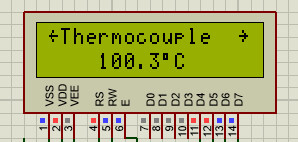
\includegraphics[scale=1]{tc_test.jpg}
        \captionof{figure}{Перевірка роботи термопари}
        \label{fig:tc_test}
    \end{minipage}
    \hspace{1em}
    \begin{minipage}{0.45\textwidth}
        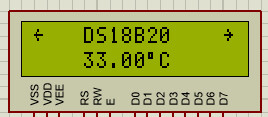
\includegraphics[scale=1]{ds18_test.jpg}
        \captionof{figure}{Перевірка роботи DS18B20}
        \label{fig:ds18_test}
    \end{minipage}
\end{figure}

\begin{figure}[ht]
    \centering
    \begin{minipage}{0.5\textwidth}
        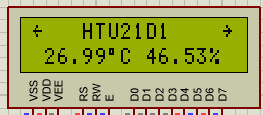
\includegraphics[scale=1]{htu21d_test.jpg}
        \captionof{figure}{Перевірка роботи HTU21D}
        \label{fig:htu21d_test}
    \end{minipage}
    \hspace{1em}
    \begin{minipage}{0.45\textwidth}
        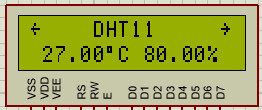
\includegraphics[scale=1]{dht11_test.jpg}
        \captionof{figure}{Перевірка роботи DHT11}
        \label{fig:dht11_test}
    \end{minipage}
\end{figure}

\begin{figure}[ht]
    \centering
    \begin{minipage}{0.5\textwidth}
        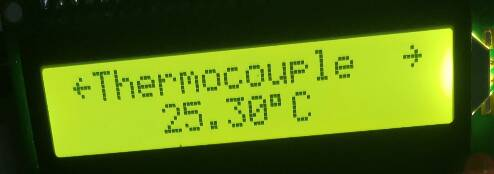
\includegraphics[width=\linewidth]{tc_test2.jpg}
        \captionof{figure}{Перевірка роботи термопари}
        \label{fig:tc_test2}
    \end{minipage}
    \hspace{1em}
    \begin{minipage}{0.45\textwidth}
        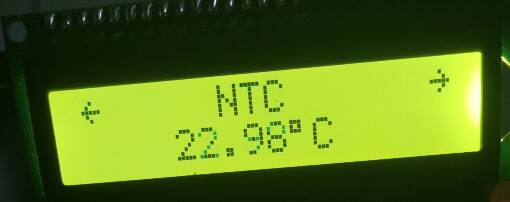
\includegraphics[width=\linewidth]{ntc_test.jpg}
        \captionof{figure}{Перевірка роботи термістору}
        \label{fig:ntc_test}
    \end{minipage}
\end{figure}

\begin{figure}[!hb]
    \centering
    \begin{minipage}{0.5\textwidth}
        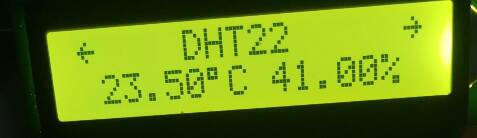
\includegraphics[width=\linewidth]{dht22_test.jpg}
        \captionof{figure}{Перевірка роботи DHT22}
        \label{fig:dht22_test}
    \end{minipage}
    \hspace{1em}
    \begin{minipage}{0.45\textwidth}
        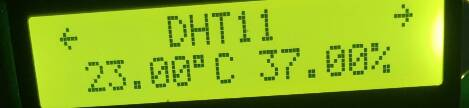
\includegraphics[width=\linewidth]{dht11_test2.jpg}
        \captionof{figure}{Перевірка роботи DHT11}
        \label{fig:dht11_test2}
    \end{minipage}
\end{figure}

\begin{figure}[H]
    \centering
    \begin{minipage}{0.5\textwidth}
        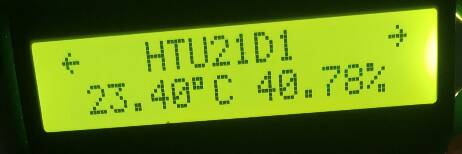
\includegraphics[width=\linewidth]{htu21d_test2.jpg}
        \captionof{figure}{Перевірка роботи HTU21D}
        \label{fig:htu21d_test2}
    \end{minipage}
    \hspace{1em}
    \begin{minipage}{0.45\textwidth}
        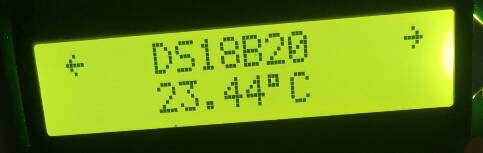
\includegraphics[width=\linewidth]{ds18_test2.jpg}
        \captionof{figure}{Перевірка роботи DS18B20}
        \label{fig:ds18_test2}
    \end{minipage}
\end{figure}



    % \AddAssociatedCounters{chapter}{appendixchapters}

\chapter{Машинний код}
\thispagestyle{headings}

\begin{lstlisting}[language={}, basicstyle=\scriptsize, caption=Машинний код]
:100000000C9426010C944E010C944E010C944E015C
:100010000C944E010C944E010C944E010C944E0124
:100020000C944E010C944E010C944E010C944E0114
:100030000C944E010C944E010C944E010C944E0104
:100040000C94C6140C944E010C9436150C94101597
:100050000C944E010C944E010C944E010C944E01E4
:100060000C94A7130C944E0108000000BE92244982
:10007000123EABAAAA2ABECDCCCC4C3E00000080DA
:10008000BEABAAAAAA3E00000000BF000000803F4D
:100090000000000000084178D3BB4387D1133D190D
:1000A0000E3CC3BD4282AD2B3E68EC8276BED98F3A
:1000B000E1A93E4C80EFFFBE01C4FF7F3F0000007E
:1000C000000000407A10F35A00A0724E1809001088
:1000D000A5D4E80000E87648170000E40B540200BD
:1000E00000CA9A3B000000E1F505000080969800E8
:1000F000000040420F000000A08601000000102711
:1001000000000000E80300000000640000000000A0
:100110000A00000000000100000000002C76D888D2
:10012000DC674F0823DFC1DFAE59E1B1B796E5E3E5
:10013000E453C63AE651997696E8E6C28426EB89FE
:100140008C9B62ED407C6FFCEFBC9C9F40F2BAA59B
:100150006FA5F490055A2AF75C936B6CF9676DC133
:100160001BFCE0E40D47FEF520E6B500D0ED902E37
:100170000300943577050080841E080000204E0A95
:10018000000000C80C333333330F986E12831141D3
:10019000EF8D2114893BE65516CFFEE6DB18D1849E
:1001A0004B381BF77C1D901DA4BBE42420328472C5
:1001B0005E228100C9F124ECA1E53D27000000008A
:1001C000240027002A0000000000250028002B0042
:1001D00000000000230026002900000000080002A3
:1001E0000100000304070000000000000000457249
:1001F000726F722100040404040404040402020265
:100200000202020303030303030102040810204057
:1002100080010204081020010204081020546865BF
:10022000726D6F636F75706C650048545532314460
:100230003100444854323200444854313100445370
:100240003138423230004E544300681511241FBE2D
:10025000CFEFD8E0DEBFCDBF11E0A0E0B1E0ECED24
:10026000F0E402C005900D92AE3DB107D9F724E04D
:10027000AEEDB1E001C01D92AE36B207E1F711E07C
:10028000C6E2D1E004C02197FE010E94711CC53274
:10029000D107C9F70E9488170C946C200C940000B9
:1002A00020911C02260F3327331F21323105ECF435
:1002B00020919802FC0190E080E0243069F082E017
:1002C0000895A0911C022191AC0146505E4FA40FED
:1002D000B52FB11D2C930196861798F380911C02BF
:1002E000680F60931C0280E0089581E008950895EE
:1002F00008950895E091F8018091F701E81730F42E
:10030000F0E0EE5AFD4F808190E008958FEF9FEF6F
:1003100008959091F8018091F7012FEF3FEF981722
:1003200048F4E92FF0E0EE5AFD4F208130E09F5F66
:100330009093F801C90108958091F7019091F80117
:10034000891B990B0895CF92DF92EF92FF920F9342
:100350001F93CF93DF937C01CB018A0120919E02F2
:10036000222389F0EB016B01C40ED51ECC15DD05EF
:1003700069F06991D701ED91FC910190F081E02D38
:10038000C7010995F3CF642F0E945001C801DF9186
:10039000CF911F910F91FF90EF90DF90CF90089534
:1003A000CF93DF931F92CDB7DEB7698320919E0272
:1003B0002223F9F02091C102203258F021E030E0F0
:1003C000FC013383228390E080E00F90DF91CF9196
:1003D000089580919F02E82FF0E0E056FD4F99814B
:1003E00090838F5F80939F028093C10281E090E0B1
:1003F000ECCF61E0CE0101960E945001F7CF682F4B
:1004000082EC92E00C94D001833081F028F48130AA
:1004100099F08230A9F008958730A9F08830C9F0AA
:100420008430B1F4809180008F7D03C08091800082
:100430008F7780938000089584B58F7784BD089569
:1004400084B58F7DFBCF8091B0008F778093B00013
:1004500008958091B0008F7DF9CFCF93DF93282F3F
:1004600030E0F901E652FE4F8491F901E75FFD4F5C
:10047000D491F901EB50FE4FC491CC23A1F081112E
:100480000E940402EC2FF0E0EE0FFF1FE053FE4F3E
:10049000A591B491EC91ED2381E090E009F480E026
:1004A000DF91CF91089580E090E0FACF1F93CF9332
:1004B000DF93282F30E0F901E652FE4F8491F901D5
:1004C000E75FFD4FD491F901EB50FE4FC491CC236F
:1004D000A9F0162F81110E940402EC2FF0E0EE0F1C
:1004E000FF1FEA53FE4FA591B4918FB7F894EC919A
:1004F000111108C0D095DE23DC938FBFDF91CF911F
:100500001F910895DE2BF8CF1092980281E080931E
:1005100097021092720261E082E10E94560261E04D
:1005200083E10E945602E9EBF0E080818E7F8083B8
:1005300080818D7F808388E48093B80085E48093F8
:10054000BC000895CF93DF9391E09093F901882345
:10055000B9F0C091B800D091BA008091BC008A7BFC
:100560008093BC0060E082E10E94560260E083E17B
:100570000E9456020E948402D093BA00C093B80031
:10058000DF91CF910895CF93DF9390E0FC01E75F77
:10059000FD4F24918B509E4FFC0184918823C9F01C
:1005A00090E0880F991FFC01E454FE4FA591B4918F
:1005B000FC01EA53FE4FC591D49161110DC09FB764
:1005C000F8948C91209582238C938881282328830A
:1005D0009FBFDF91CF910895623051F49FB7F89497
:1005E0003C91822F809583238C93E8812E2BEFCF33
:1005F0008FB7F894EC912E2B2C938FBFEACFBF923C
:10060000CF92DF92EF92FF920F931F93CF93DF93DE
:10061000D82FC8E09BEEE92EF12C2FE0C22ED12C72
:1006200061E083E00E94C302BFB6F8940D2F10E092
:10063000D0FF1AC0C6010197F1F760E083E00E9485
:10064000C302C7010197F1F7BFBE15950795D02FDB
:10065000C15031F7DF91CF911F910F91FF90EF9033
:10066000DF90CF90BF900895C7010197F1F760E048
:1006700083E00E94C302C601E5CF1F93CF93DF93AF
:1006800061E083E00E94C302CBE5D9E0CE0101978F
:10069000F1F760E083E00E94C3021FB7F8948BEE8D
:1006A00090E00197F1F783E00E942D029C011FBFAB
:1006B0002197F1F781E0232B09F080E0DF91CF91C2
:1006C0001F9108952F923F924F925F926F927F9267
:1006D0008F929F92AF92BF92CF92DF92EF92FF9252
:1006E0000F931F93CF93DF9300D000D0CDB7DEB729
:1006F0008C0181E0F80180830E943D03382E811136
:1007000019C0312C832D0F900F900F900F90DF9117
:10071000CF911F910F91FF90EF90DF90CF90BF90FE
:10072000AF909F908F907F906F905F904F903F9091
:100730002F9008958CEC0E94FF028EEB0E94FF0226
:100740001982712C612C412C43E0842E912C5BE1A9
:10075000C52ED12C6BEEA62EB12C38E0232E512CB9
:10076000E52CF12CF594E7945E2CFFB7FA83F8940E
:1007700061E083E00E94C302C4010197F1F760E0E9
:1007800083E00E94C302C6010197F1F783E00E9453
:100790002D02892B11F0689457F8C5010197F1F7E4
:1007A0002A812FBF2A942110DBCF252D30E0620E45
:1007B000731E8981852598E04CE8869508F4842786
:1007C0009A95D9F7898341101CC03C832B834394AD
:1007D000F9E04F12C2CF27EF621628E0720609F443
:1007E00090CF672809F48DCF81118BCF4B815C812D
:1007F000403585E0580709F485CFF80152834183DD
:1008000081CF41E04412E3CF322F2227EB81FC81DC
:10081000E22BF32BFC83EB83DACF8E508064809342
:100820007C0080917A00806480937A0080917A00C5
:1008300086FDFCCF809178009091790008953FB7B4
:10084000F8948091F3019091F401A091F501B09199
:10085000F60126B5A89B05C02F3F19F00196A11DF2
:10086000B11D3FBFBA2FA92F982F8827BC01CD01FA
:10087000620F711D811D911D42E0660F771F881F59
:10088000991F4A95D1F708958F929F92AF92BF9288
:10089000CF92DF92EF92FF920F931F93CF93DF934C
:1008A000D091C102D13208F0D7C0182FC091C00238
:1008B0000E941F046B017C018091980281116BC022
:1008C00082E080939802109397028FEF80939602B4
:1008D00010929502D0939402A0EAB2E0E4E7F2E02D
:1008E00080E0D81391C01092730280917302CC0FF4
:1008F000C82BC093730280917202813009F088C0C6
:10090000109272020E941F046B017C01809173029D
:100910008093BB0080919A0290919B02A0919C02CF
:10092000B0919D02892B8A2B8B2BA1F00E941F0472
:1009300000919A0210919B0220919C0230919D029D
:100940006C197D098E099F090617170728073907B3
:1009500008F442C08091BC0083FDD8CF85EC809321
:10096000BC000E941F046B017C01809198028230C0
:1009700009F450C0809196028F3F09F46FC08091B6
:100980009602803209F46CC080919602803309F49B
:1009900069C084E026C080919A0290919B02A09148
:1009A0009C02B0919D02892B8A2B8B2B09F484CF5A
:1009B0000E941F0480909A0290909B02A0909C023B
:1009C000B0909D026C197D098E099F0986169706C5
:1009D000A806B90608F070CF809199020E94A20281
:1009E00085E010929F021092C10210929E02DF9148
:1009F000CF911F910F91FF90EF90DF90CF90BF901C
:100A0000AF909F908F9008959D9191938F5F69CF44
:100A100085EEA5CF80919A0290919B02A0919C02B5
:100A2000B0919D02892B8A2B8B2B09F49ECF0E94BB
:100A30001F0400919A0210919B0220919C02309118
:100A40009D026C197D098E099F0906171707280753
:100A5000390708F08ACFC0CF81E0C3CF80E0C1CF93
:100A600082E0BFCF83E0BDCFCF92DF92EF92FF92C3
:100A70000F931F93CF93DF93D82FC62F613208F0C7
:100A800098C00E941F046B017C0180919802811123
:100A90006BC081E080939802809397029FEF9093C0
:100AA0009602109295029C0F909394028093730289
:100AB00080917302DD0FD82BD09373028091720264
:100AC000813009F078C0109272020E941F046B01FD
:100AD0007C01809173028093BB0080919A02909177
:100AE0009B02A0919C02B0919D02892B8A2B8B2B9B
:100AF000A1F00E941F0400919A0210919B02209184
:100B00009C0230919D026C197D098E099F09061780
:100B100017072807390708F448C08091BC0083FDF7
:100B2000D8CF85EC8093BC000E941F046B017C0130
:100B300080919802813009F440C0809195028C1711
:100B400010F4C0919502E4E7F2E0A2E5B2E080E0A3
:100B50008C1355C08C2FDF91CF911F910F91FF9077
:100B6000EF90DF90CF90089580919A0290919B0230
:100B7000A0919C02B0919D02892B8A2B8B2B09F4AA
:100B800084CF0E941F0400919A0210919B02209131
:100B90009C0230919D026C197D098E099F090617F0
:100BA00017072807390708F070CF809199020E9433
:100BB000A202C0E0CFCF85EEB5CF80919A0290918E
:100BC0009B02A0919C02B0919D02892B8A2B8B2BBA
:100BD00009F4AECF0E941F0400919A0210919B026B
:100BE00020919C0230919D026C197D098E099F090C
:100BF000061717072807390708F09ACFD6CF919123
:100C00009D938F5FA5CF8F929F92AF92BF92CF920D
:100C1000DF92EF92FF926B017C010E941F044B0157
:100C20005C01C114D104E104F104B9F00E941F0475
:100C3000681979098A099B09683E73408105910505
:100C400080F321E0C21AD108E108F10888EE880E8D
:100C500083E0981EA11CB11CE4CFFF90EF90DF90C1
:100C6000CF90BF90AF909F908F9008952FB7F8943A
:100C70006091EF017091F0018091F1019091F2018A
:100C80002FBF0895AF92BF92CF92DF92EF92FF9263
:100C90000F931F93CF93DF936C017B018B01040FA4
:100CA000151FEB015E01AE18BF08C017D10759F040
:100CB0006991D601ED91FC910190F081E02DC60182
:100CC0000995892B79F7C501DF91CF911F910F917C
:100CD000FF90EF90DF90CF90BF90AF900895FC0110
:100CE000538D448D252F30E0842F90E0821B930B91
:100CF000541710F0CF96089501970895FC01918D37
:100D0000828D981761F0A28DAE0FBF2FB11D5D9639
:100D10008C91928D9F5F9F73928F90E008958FEFDB
:100D20009FEF0895FC01918D828D981731F0828D8F
:100D3000E80FF11D858D90E008958FEF9FEF0895E6
:100D4000FC01918D228D892F90E0805C9F4F821B4A
:100D500091098F73992708958EEC92E00E94A00666
:100D600021E0892B09F420E0822F089580E090E0B3
:100D7000892B29F00E94AC0681110C940000089583
:100D8000FC01A48DA80FB92FB11DA35ABF4F2C9100
:100D9000848D90E001968F739927848FA689B789F7
:100DA0002C93A089B1898C91837080648C93938DEE
:100DB000848D981306C00288F389E02D80818F7D91
:100DC00080830895EF92FF920F931F93CF93DF9349
:100DD000EC0181E0888F9B8D8C8D98131AC0E88977
:100DE000F989808185FF15C09FB7F894EE89FF8946
:100DF0006083E889F98980818370806480839FBFE4
:100E000081E090E0DF91CF911F910F91FF90EF90E3
:100E10000895F62E0B8D10E00F5F1F4F0F731127F3
:100E2000E02E8C8D8E110CC00FB607FCFACFE8892E
:100E3000F989808185FFF5CFCE010E94C006F1CFF0
:100E4000EB8DEC0FFD2FF11DE35AFF4FF0829FB7A2
:100E5000F8940B8FEA89FB8980818062CFCFCF9392
:100E6000DF93EC01888D8823B9F0AA89BB89E889D2
:100E7000F9898C9185FD03C0808186FD0DC00FB678
:100E800007FCF7CF8C9185FFF2CF808185FFEDCFF6
:100E9000CE010E94C006E9CFDF91CF910895FC01F9
:100EA000248131E030939E022093C00210929F0271
:100EB0001092C1028485862B90E00E94FF0181E0A0
:100EC0000C944404089590E080E00895CF93C42FDB
:100ED000FC01828191E090939E028093C002109267
:100EE0009F021092C10282EC92E00E94D0016C2F0E
:100EF00082EC92E00E94D00181E00E94440491E0E3
:100F0000811101C090E0892F8195CF910895CF92F2
:100F1000DF92EF92FF92CF93DF93DC011796CC9193
:100F20001797D0E06111DC2F18962C91189730E0BC
:100F3000220F331F20533E4F50E040E0F9018591CE
:100F40009491FC01F080BA0190E080E0EF2DEC2359
:100F5000ED1310C04F5F5F4F1D96CD90DD90ED906B
:100F6000FC9050976C157D058E059F0538F36FEF4B
:100F70007FEFCB01DF91CF91FF90EF90DF90CF908B
:100F800008958F929F92AF92BF92CF92DF92EF928D
:100F9000FF920F931F93CF93DF93CDB7DEB7C0546B
:100FA000D1400FB6F894DEBF0FBECDBF8C010E94BA
:100FB0003606F801C184D284E384F4849B01AC0139
:100FC0002C193D094E095F0969017A0130EDC316FC
:100FD00037E0D306E104F104A8F48189C05CDE4F58
:100FE0000FB6F894DEBF0FBECDBFDF91CF911F913A
:100FF0000F91FF90EF90DF90CF90BF90AF909F90B8
:101000008F900895618772878387948714821382F3
:1010100012821182108262E085810E94C30261E027
:1010200070E080E090E00E94030661E0F8018581B5
:101030000E94C30260E0F80185810E945602F80117
:1010400086818551823028F58BE291E10197F1F795
:1010500062E0F80185810E94C302F801828990E074
:101060008230910538F0880F991F880F991F0597D6
:101070000197F1F7F89460E0C8010E9487076F3F7D
:101080007F4F8F4F9F4F61F4F801118A789480E071
:10109000A5CF64E170E080E090E00E940306D8CF25
:1010A00061E0C8010E9487076F3F7F4F8F4F9F4FBE
:1010B00059F39E012F5F3F4F79015E013FEBA31A69
:1010C0003EEFB30A670160E0C8010E948707F6019E
:1010D000608371838283938361E0C8010E948707E4
:1010E000F6016483758386839783F8E0CF0ED11C65
:1010F000CA14DB0441F7789430E020E0F7018080E7
:101100009180A280B3804481558166817781FFEF11
:101110008F169F06AF06BF0631F04F3F8FEF58077F
:101120006807780719F4F801118AB1CFF90183E053
:10113000F595E7958A95E1F7E00FF11F8081880F1B
:1011400084169506A606B706F0F080832F5F3F4F02
:10115000F8E0EF0EF11C2832310581F6F8014481E8
:1011600020818181280F3327331F8281280F311D71
:101170008381820F932F911D99274817190699F69D
:1011800081E0818B2BCF8160E0CFFC0183898B30A4
:1011900051F480E492E4AFE0B0E0FB0184A395A3B6
:1011A000A6A3B7A3089580E894E8AEE1B0E0F5CF38
:1011B00090E080E00895CF92DF92EF92FF920F933C
:1011C0001F93CF93DF93EC018B017A018E859F856E
:1011D0000E946203882309F443C0CE84DF84F601B1
:1011E0008081811103C0C6010E946203F601618102
:1011F0007281072E000C880B990B0E948C1D20E039
:1012000030E040E85DE30E94911EF8016083718345
:1012100082839383E114F10449F080E090E0A0E838
:10122000BFEBF70180839183A283B383F8018081B0
:101230009181A281B3818E839F83A887B98780E043
:1012400090E0A0E8BFEB8A879B87AC87BD87DF91E2
:10125000CF911F910F91FF90EF90DF90CF90089565
:101260006E817F8188859985D0CF81E090E0089557
:10127000DC011E96ED91FC9110820E943D038823B3
:1012800031F08CEC0E94FF0284E40E94FF0281E0B6
:10129000089582E090E00895CF93DF93FC01C68526
:1012A000D78562E08D810E94C3020E943606605D90
:1012B00077408109910969877A878B879C8787E3C3
:1012C0008A8B81E0DF91CF91089583E090E00895CB
:1012D000CF93DF93FC01C685D78562E08D810E94A4
:1012E000C3020E943606605D7740810991096987D3
:1012F0007A878B879C8787E38A8B81E0DF91CF9108
:10130000089584E090E008958F929F92AF92BF92EB
:10131000CF92DF92EF92FF920F931F93CF93DF93C1
:1013200000D000D0CDB7DEB78C016B017A01DC01B3
:101330001E968D919C91DC01ED91FC910680F781C8
:10134000E02D50E040E0BE016F5F7F4F099581E1E5
:101350000E940D04BC0190E080E00E948A1D20E004
:1013600030E040EA5BE30E94911E4B015C0129E200
:101370003CE54FE05DE30E94E41C87FD5BC079E241
:101380006CE59FE08DE3272F362F492F582FB401AE
:10139000C5010E94771C4B015C0120E030E04CE568
:1013A00053E4F80160897189828993890E94911EB2
:1013B0009B01AC01C501B4010E94E91C29813A815D
:1013C0004B815C810E94781CD6016D937D938D9337
:1013D0009C931397E114F10449F080E090E0A0E8B9
:1013E000BFEBF70180839183A283B383F7018081F0
:1013F0009181A281B381F601408151816281738123
:10140000F801468357836087718782879387A48713
:10141000B5870F900F900F900F90DF91CF911F9194
:101420000F91FF90EF90DF90CF90BF90AF909F9083
:101430008F900895782D692D9A2D8B2DA4CF85E05E
:1014400090E00895DC011E968D919C91DC01ED9158
:10145000FC910190F081E02D099408958F929F9264
:10146000AF92BF92CF92DF92EF92FF921F93CF93F2
:10147000DF93FC01108511110EC010E0812FDF9168
:10148000CF911F91FF90EF90DF90CF90BF90AF90E2
:101490009F908F900895EC010E943606C880D980F5
:1014A000EA80FB804B015C018C189D08AE08BF08E8
:1014B000CC80DD80EE80FF80C814D904EA04FB04F0
:1014C000E0F6688379838A839B83E985FA85309780
:1014D000A9F28B859C850995D1CF81E00895089567
:1014E000FB0101900020E9F73197AF01461B570B34
:1014F000DC01ED91FC910280F381E02D09948F9243
:101500009F92AF92BF920F931F93CF93DF93CDB76C
:10151000DEB7A1970FB6F894DEBF0FBECDBF19A2FC
:10152000423008F44AE08E010F5D1F4F842E912C4B
:10153000B12CA12CA50194010E944F1CE62FB901EA
:10154000CA01EA3004F5E05DD801EE938D01232B4A
:10155000242B252B79F790E080E0109729F0BD012E
:101560008EEC92E00E94700AA1960FB6F894DEBF4E
:101570000FBECDBFDF91CF911F910F91BF90AF9064
:101580009F908F900895E95CDFCFCF92DF92EF922A
:10159000FF920F931F93CF93DF938C01EB01FB011D
:1015A000349680E2DF011D928A95E9F784E290E0AB
:1015B000A0E0B0E088839983AA83BB83F80184818B
:1015C0009581A681B7818C839D83AE83BF838CE098
:1015D00090E0A0E0B0E088879987AA87BB870E9447
:1015E0003606688B798B8A8B9B8BD80112960D916E
:1015F0001C91C8010E94C107882349F0F801868127
:101600008B3028F08D3040F08551823070F160E0F1
:1016100070E080EC9FE71BC0618170E090E080E0AB
:101620000E948C1D2DEC3CEC4CEC5DE30E94911E65
:101630006B017C01F801608170E090E080E00E9425
:101640008C1D9B01AC01C701B6010E94781C6C8BFC
:101650007D8B8E8B9F8B81E0DF91CF911F910F91BE
:10166000FF90EF90DF90CF90089560817181762791
:101670006727762790E080E00E948A1D2DEC3CECE5
:101680004CEC5DE30E94911EE2CF8F929F92AF924D
:10169000BF92EF92FF921F93CF93DF937C01EB01F8
:1016A000FB01349680E2DF011D928A95E9F784E21E
:1016B00090E0A0E0B0E088839983AA83BB83F70120
:1016C00084819581A681B7818C839D83AE83BF83FE
:1016D0008DE090E0A0E0B0E088879987AA87BB877B
:1016E0000E943606688B798B8A8B9B8BD70112966A
:1016F000ED90FC90C7010E94C107882341F0F701DB
:1017000086818C3009F455C038F48B30E1F060E00C
:1017100070E080EC9FE73EC085518230C0F71281B7
:10172000612F70E0762F662766277F778381682B8D
:1017300090E080E00E948A1D2DEC3CEC4CEC5DE3D7
:101740000E94911E51C0628170E090E080E00E9492
:101750008A1D4B015C01F701138117FF0AC0AC0120
:101760009B0160E070E080E89FEB0E94771C4B01DA
:101770005C011F70612F70E090E080E00E948C1D82
:101780002DEC3CEC4CEC5DE30E94911EA501940114
:101790000E94781C6C8B7D8B8E8B9F8B81E0DF9100
:1017A000CF911F91FF90EF90BF90AF909F908F903F
:1017B00008951281612F70E090E080E00E948A1D00
:1017C0004B015C01F70163816F7070E090E080E095
:1017D0000E948C1D2DEC3CEC4CEC5DE30E94911EB4
:1017E000A50194010E94781C17FFD4CF9058D2CF46
:1017F000CF92DF92EF92FF920F931F93CF93DF93DD
:10180000CDB7DEB7AC970FB6F894DEBF0FBECDBF35
:101810008C016B017A01DC011E96ED91FC918CE547
:1018200091E09EA38DA38689978998A78FA3808D29
:10183000918DA28DB38D89A79AA7ABA7BCA7BE0136
:101840006F5F7F4FCE0185960E94450B8D899E89E3
:10185000AF89B88DF60180839183A283B383D801C9
:101860001E96ED91FC918EE491E09EA38DA3868D52
:10187000978D98A78FA380A191A1A2A1B3A189A7B9
:101880009AA7ABA7BCA7BE016F5F7F4FCE0185961D
:101890000E94C50AE114F10449F08D899E89AF893F
:1018A000B88DF70180839183A283B383F701808190
:1018B0009181A281B381F60140815181628173815E
:1018C000F801468357836087718782879387A4874F
:1018D000B587AC960FB6F894DEBF0FBECDBFDF91D3
:1018E000CF911F910F91FF90EF90DF90CF900895CF
:1018F000CF92DF92EF92FF920F931F93CF93DF93DC
:10190000CDB7DEB7AC970FB6F894DEBF0FBECDBF34
:101910008C016B017A01DC011E96ED91FC918CE546
:1019200091E09EA38DA38689978998A78FA3808D28
:10193000918DA28DB38D89A79AA7ABA7BCA7BE0135
:101940006F5F7F4FCE0185960E94450B8D899E89E2
:10195000AF89B88DF60180839183A283B383D801C8
:101960001E96ED91FC918EE491E09EA38DA3868D51
:10197000978D98A78FA380A191A1A2A1B3A189A7B8
:101980009AA7ABA7BCA7BE016F5F7F4FCE0185961C
:101990000E94C50AE114F10449F08D899E89AF893E
:1019A000B88DF70180839183A283B383F70180818F
:1019B0009181A281B381F60140815181628173815D
:1019C000F801468357836087718782879387A4874E
:1019D000B587AC960FB6F894DEBF0FBECDBFDF91D2
:1019E000CF911F910F91FF90EF90DF90CF900895CE
:1019F00085ED8093BC0080919A0290919B02A0910A
:101A00009C02B0919D020796A11DB11D23E0B695E1
:101A1000A795979587952A95D1F72091BC0024FD2D
:101A200003C010929802089540919A0250919B022F
:101A300060919C0270919D02452B462B472B69F3C8
:101A40000097A105B10541F025E32A95F1F70000C3
:101A50000197A109B109E1CF809199020C94A202EA
:101A60000F931F93CF938C01C62F0E944F076C2FAB
:101A70006460C8010E944F076C2F6B7FC8010E94F1
:101A80004F0783EC90E00197F1F7CF911F910F91F1
:101A900008950F931F93CF93DF938C01D62FC42FFC
:101AA000607F642B0E94300D80E1D89FB00111242B
:101AB0006C2BC801DF91CF911F910F910C94300DC9
:101AC00041E00E94490D81E090E00895CF93DF93BB
:101AD000CDB7DEB728970FB6F894DEBF0FBECDBFE7
:101AE00028E0E6E0F1E0DE01119601900D922A95E2
:101AF000E1F7FC012085241708F44FEF50E0440F74
:101B0000551F21E030E02C0F3D1F420F531FFA01FB
:101B10002081620F606840E028960FB6F894DEBF1F
:101B20000FBECDBFDF91CF910C94490DCF93DF93C2
:101B3000C0E9D3E040E060E0888199810E94660DB1
:101B400041E06FE785EA93E00E94490D40E06FE0D5
:101B5000888199810E94660D41E06EE785EA93E0F5
:101B6000DF91CF910C94490D8F929F92AF92BF92CB
:101B7000CF92DF92EF92FF920F931F934B015C0184
:101B800069017A0141E060E08091900390919103B6
:101B90000E94660DE2E9F3E081E1DF011D928A9582
:101BA000E9F71092A30311E01093A403A501940197
:101BB000C501B4010E94FE1E882311F141E150E0ED
:101BC0006EEE71E082E993E00E94D21920E030E0ED
:101BD00040E85FEBC701B6010E94E41C882309F4CA
:101BE00055C08091A40381113CC01F910F91FF90BB
:101BF000EF90DF90CF90BF90AF909F908F9008951F
:101C00001093A30380E28093920303E913E022E0A0
:101C100045E0C501B4010E94AB19E091A303A5E022
:101C2000AE0FA093A3038091A403882379F2B0E0C0
:101C3000A057BC4F8FED12968C9387E08E0F809348
:101C4000A303EA5FF0E0E057FC4F83E4828320E0E7
:101C500030E040E85FEBC701B6010E94E41C882336
:101C6000D1F00091A303A7019601C701B6010E941C
:101C7000FE1E202F30E0882329F141E150E06EEE76
:101C800071E0C9018E569C4F0E94D2198091A40325
:101C9000882309F4AACF8091A303869567E0681B87
:101CA00041E080919003909191030E94660D62E95A
:101CB00073E080919003909191030E94700A1092BA
:101CC000A40393CF0F5F0093A30320573C4F80E200
:101CD000F901828310E00E561C4F22E045E0C70157
:101CE000B6010E94AB198091A303E5E0E80FE093F1
:101CF000A3039091A403992309F477CF8A5F80937B
:101D0000A303F0E0E057FC4F85E28283BFCFCF937F
:101D1000DF93EC0140E061E00E94490D8BE39FE11D
:101D20000197F1F78985882339F040E060E0CE0122
:101D3000DF91CF910C94660DDF91CF9108950F93B1
:101D40001F93CF93DF938C0141E150E0BC0181E40C
:101D500092E00E94D219C0E9D3E0888199810E9463
:101D6000870EC8010E94C9199695879567E0681B80
:101D700040E0888199810E94660D61E472E088816B
:101D80009981DF91CF911F910F910C94700ACF939D
:101D9000DF93EC018A8191E090939E028093C002D0
:101DA00010929F021092C10282EC92E00E94D00138
:101DB00081E00E944404882321F08FEFDF91CF91CE
:101DC000089561E08A810E9434051092F8018093A1
:101DD000F701813091F782EC92E00E948901EECF09
:101DE0008F929F92AF92BF92CF92DF92EF92FF922B
:101DF0000F931F93CF93DF938C016B017A01FC014A
:101E0000C685D7858A8191E090939E028093C00217
:101E100010929F021092C10283EE90E00E94FF0197
:101E200081E00E944404882309F44EC060E070E021
:101E30008FE793E4F6016083718382839383F801D3
:101E4000C685D7858A8191E090939E028093C002D7
:101E500010929F021092C10285EE90E00E94FF0155
:101E600081E00E944404882309F484C0812C912CD1
:101E70005FE7A52E53E4B52EE114F10429F0F70134
:101E800080829182A282B382F70180819181A281B6
:101E9000B381F6014081518162817381F8014683EB
:101EA00057836087718782879387A487B587DF917F
:101EB000CF911F910F91FF90EF90DF90CF90BF9047
:101EC000AF909F908F90089588816BE2803839F0B1
:101ED0006BE0813821F065E5813009F466E170E05E
:101EE00090E080E00E94030663E08A810E9434054E
:101EF0001092F8018093F701833009F097CF82ECBC
:101F000092E00E948901A12CB82E82EC92E00E94FE
:101F10008901A82AB92AE50180E19E01CC0FDD1FC5
:101F200037FF02C0F1E3DF278150B9F782EC92E07E
:101F30000E948901CD2FDD27C817D90709F076CF78
:101F40008CEFA822B50190E080E00E948A1D22E576
:101F500038EB4FE253E40E94911E20E030E040E86D
:101F600057E30E94911E26E636E64BE352E40E94B8
:101F7000771C60CF88816DE0803839F06FE0813860
:101F800021F06DE1813009F467E070E090E080E0DD
:101F90000E94030663E08A810E9434051092F801D2
:101FA0008093F701833009F061CF82EC92E00E94C8
:101FB0008901A12CB82E82EC92E00E948901A82A06
:101FC000B92AE50180E19E01CC0FDD1F37FF02C079
:101FD000F1E3DF278150B9F782EC92E00E9489019A
:101FE000CD2FDD27C817D90709F040CF8CEFA822E5
:101FF000B50190E080E00E948A1D20E030E04AEFC9
:1020000052E40E94911E20E030E040E857E30E9435
:10201000911E20E030E040EC50E40E94771C4B0120
:102020005C0120E030E0A9010E94E41C87FD12C0A1
:1020300020E030E048EC52E4C501B4010E943C1EAF
:1020400018160CF019CF812C912C88ECA82E82E464
:10205000B82E12CF812C912C54010ECF1F93CF9309
:10206000DF93FC01C685D7851092F8011092F70125
:1020700010929F021092C1020E94840287E791E0B1
:1020800090931B0280931A0288E791E090931F02BD
:1020900080931E0288E48093B8001092F90188EEC4
:1020A00093E0A0E0B0E080939A0290939B02A0930B
:1020B0009C02B0939D02109299028981823038F07F
:1020C000853058F460E570E080E090E004C06FE097
:1020D00070E080E090E00E9403068A8111E0109396
:1020E0009E028093C00210929F021092C10281E072
:1020F0000E944404882329F080E0DF91CF911F9152
:1021000008958A8110939E028093C00210929F02CC
:102110001092C1028EEF90E00E94FF0181E00E94C8
:1021200044046FE070E080E090E00E94030667EEF8
:10213000CE010E94C70E8F3F31F0482F4B7F66EED5
:10214000CE010E946607188167EECE010E94C70E7D
:102150008F3F51F08E77412F482B66EECE010E94C3
:1021600066078F3F09F0188367EECE010E94C70E05
:102170008F3F11F286FB882780F991E08927BDCF38
:102180004F925F926F927F92AF92BF92CF92DF9207
:10219000EF92FF920F931F93CF9386E6A82E81E0D4
:1021A000B82EC0E0D5010D911D915D01D801ED91D2
:1021B000FC910680F781E02D4EED51E062EE71E07A
:1021C000C8010995C090E201D090E301E090E401DC
:1021D000F090E501A7019601C701B6010E94FE1E1D
:1021E0006EEA71E081111BC026013701E89477F88F
:1021F0002FEF3FEF4FE75FE7C301B2010E94FE1EE2
:10220000811159C02FEF3FEF4FE75FE7C301B201E4
:102210000E94E41C18160CF04EC062EB71E08EECCC
:1022200092E00E94700AC53031F06AEB71E08EECEA
:1022300092E00E94700AD801ED91FC910280F38136
:10224000E02DC8010995CF5FC63009F0ABCF6DEB2B
:1022500071E08EEC92E00E94700A80918D03909163
:102260008E03DC01ED91FC910680F781E02D4EEDAF
:1022700051E062EE71E009952091DE013091DF01BD
:102280004091E0015091E1016091E2017091E30120
:102290008091E4019091E501CF911F910F91FF9002
:1022A000EF90DF90CF90BF90AF907F906F905F9056
:1022B0004F900C94B40D2FEF3FEF4FE75FE4C70151
:1022C000B6010E943C1E18161CF466EB71E0A7CF05
:1022D0002FEF3FEF4FE75FECC701B6010E94E41C10
:1022E00087FDF3CF20E030E0A901C701B6010E94CD
:1022F000E41C87FF09C06DE28EEC92E00E94E206CA
:10230000F7FAF094F7F8F0942AE037ED43EA5BE34C
:10231000C701B6010E94781C2B013C010E945B1D85
:102320006B017C010E948A1D9B01AC01C301B201BB
:102330000E94771C2B013C014AE0C701B6010E94B4
:102340007F0A6EE28EEC92E00E94E20620E030E02E
:1023500040E251E4C301B2010E94911E2B013C01F5
:102360000E945B1D6B01F12CE12C4AE0C701B60114
:102370000E947F0AC701B6010E948A1D9B01AC0121
:10238000C301B2010E94771C20E030E040E251E43A
:102390000E94911E0E945B1D90E080E04AE00E9436
:1023A0007F0A41CFCF93DF93EB01FC0183894BE0A0
:1023B00050E066EC71E08C30C1F058F44BE050E036
:1023C00060EC71E08B3089F04BE050E068ED71E03B
:1023D0000CC04BE050E06CEC71E0853131F04BE02B
:1023E00050E062ED71E0863179F7CE010E945D2008
:1023F0001B86DF91CF9108950F931F93CF93DF93A7
:102400008C01EB0188E2DB011D928A95E9F7F80166
:10241000828193810E94D21181E090E0A0E0B0E03F
:102420008C879D87AE87BF87F80184819581A681BF
:10243000B781888B998BAA8BBB8B8CE090E0A0E056
:10244000B0E08C8B9D8BAE8BBF8BBE018281938164
:102450000E94C508D8011296ED91FC9183898C30B9
:1024600009F441C078F48B3009F1188E198E1A8E58
:102470001B8E1C8E1D8E1E8E1F8E18A219A21AA2D4
:102480001BA22CC08551823080F780E090E0A8EC40
:10249000B2E4888F998FAA8FBB8F1C8E1D8E1E8EE3
:1024A0001F8E8DEC9CECACECBDE314C080E090E0A2
:1024B000A0EAB2E4888F998FAA8FBB8F80E090E06A
:1024C000A0EAB1E48C8F9D8FAE8FBF8F80E090E04B
:1024D000A0EAB0E488A399A3AAA3BBA3DF91CF91FC
:1024E0001F910F91089580E090E0AEEBB2E4E2CF4F
:1024F0000F931F93CF93DF938C01EB0188E2DB01F5
:102500001D928A95E9F7F801828193810E94D21188
:1025100081E090E0A0E0B0E08C879D87AE87BF8728
:10252000F80184819581A681B781888B998BAA8BCC
:10253000BB8B8DE090E0A0E0B0E08C8B9D8BAE8BF0
:10254000BF8BBE01828193810E94C508D80112967B
:10255000ED91FC9183898C3091F178F48B30B1F05E
:10256000188E198E1A8E1B8E1C8E1D8E1E8E1F8E1F
:1025700018A219A21AA21BA21DC08531A9F1863189
:1025800079F780E090E0AAEFB2E432C080E090E01A
:10259000A8E4B2E4888F998FAA8FBB8F1C8E1D8E02
:1025A0001E8E1F8E80E090E0A0E0B0E488A399A387
:1025B000AAA3BBA3DF91CF911F910F91089580E053
:1025C00090E0A0E7B2E4888F998FAA8FBB8F80E05C
:1025D00090E0A0EAB1EC8C8F9D8FAE8FBF8F80E032
:1025E00090E0A0E0BFE3E2CF80E090E0A0EAB2E4B8
:1025F000888F998FAA8FBB8F80E090E0A0E2B2EC29
:102600008C8F9D8FAE8FBF8F8DEC9CECACECBDE3BF
:10261000CDCF4F925F926F927F928F929F92AF92A7
:10262000BF92CF92DF92EF92FF920F931F93CF93BF
:10263000DF93EC018B017A01CE84DF8480E4982E55
:10264000B12CA12C8EE00E940D04A80EB91E9A9404
:102650009110F8CFB50190E080E00E948A1D20E043
:1026600030E040E85CE30E94911E0E945B1D90E018
:1026700080E00E948A1D4B015C01F60120813181BE
:10268000428153810E94911E2B013C01A5019401BE
:1026900060E070EC8FE794E40E94771C9B01AC0132
:1026A000C301B2010E94E91C0E94491E20E030EEE5
:1026B00046E755E40E94E91C2FE03FEC4BE55BE365
:1026C0000E94781C9B01AC0160E070E080E89FE311
:1026D0000E94E91C23E333E948E853E40E94771C95
:1026E000F8016083718382839383E114F10449F0DC
:1026F00080E090E0A0E8BFEBF70180839183A283A4
:10270000B383F80180819181A281B3818E839F83FD
:10271000A887B98780E090E0A0E8BFEB8A879B8715
:10272000AC87BD87DF91CF911F910F91FF90EF9004
:10273000DF90CF90BF90AF909F908F907F906F90E1
:102740005F904F9008950C94D41F0C94D41F1F9247
:102750000F920FB60F9211242F933F934F935F93D5
:102760006F937F938F939F93AF93BF93EF93FF9359
:102770008091B900887F803609F44AC0F0F588322C
:1027800009F4A7C018F5803109F49BC0B8F4882378
:1027900009F4F9C0883009F494C0FF91EF91BF911A
:1027A000AF919F918F917F916F915F914F913F91E9
:1027B0002F910F900FBE0F901F901895883109F43C
:1027C00088C0803251F78093960214C0803409F497
:1027D0009DC040F48033B9F38833F9F680939602B4
:1027E00085ECB0C0803509F485C0883509F496C001
:1027F000883499F60E94F80CD0CF883909F48CC03F
:1028000038F5883729F050F4883611F0803729F6EA
:1028100083E0809398021092400257C0883809F4F0
:102820007BC0803919F0803809F0B7CF8091400221
:10283000803208F071C0E091400281E08E0F8093F9
:1028400040028091BB00F0E0E05EFD4F80833DC020
:10285000803B39F0E0F4803A09F479C0883A09F015
:102860009CCF84E08093980210921D0210921C026B
:10287000E0911A02F0911B02099580911C028111CE
:102880000FC081E080931C021092FA0109C0803CC5
:1028900009F4A6CF883C09F4A3CF883B09F07DCF8B
:1028A000E0911D0281E08E0F80931D02F0E0E65062
:1028B000FE4F80818093BB0090911D0280911C028D
:1028C00029C0809173028093BB0085EC8093BC008B
:1028D00064CF9091950280919402981758F5E091F9
:1028E000950281E08E0F80939502F0E0EC58FD4F49
:1028F0008081E9CFE091950281E08E0F809395026F
:102900008091BB00F0E0EC58FD4F808390919502E0
:10291000809194029817C8F285E8D8CFE09195028B
:1029200081E08E0F809395028091BB00F0E0EC581F
:10293000FD4F80838091970281115CCF81E080936D
:10294000720284EA8093BC001092980226CF85EC34
:102950008093BC001092980280914002803230F443
:10296000E0914002F0E0E05EFD4F10826091400295
:1029700070E0E0911E02F0911F0280E292E0099562
:10298000109240020ACF1092960234CF1F920F92FB
:102990000FB60F9211242F933F938F939F93AF9372
:1029A000BF938091EF019091F001A091F101B0915E
:1029B000F2013091EE0123E0230F2D3758F50196F7
:1029C000A11DB11D2093EE018093EF019093F001C2
:1029D000A093F101B093F2018091F3019091F40181
:1029E000A091F501B091F6010196A11DB11D809352
:1029F000F3019093F401A093F501B093F601BF9118
:102A0000AF919F918F913F912F910F900FBE0F909B
:102A10001F90189526E8230F0296A11DB11DD2CF55
:102A20001F920F920FB60F9211242F933F934F9343
:102A30005F936F937F938F939F93AF93BF93EF9326
:102A4000FF938EEC92E00E94C006FF91EF91BF9140
:102A5000AF919F918F917F916F915F914F913F9136
:102A60002F910F900FBE0F901F9018951F920F92ED
:102A70000FB60F9211242F938F939F93EF93FF9391
:102A8000E091DE02F091DF028081E091E402F091BA
:102A9000E50282FD1BC090818091E7028F5F8F73FA
:102AA0002091E802821741F0E091E702F0E0E25362
:102AB000FD4F958F8093E702FF91EF919F918F914A
:102AC0002F910F900FBE0F901F9018958081F4CF1B
:102AD0002F923F924F925F926F927F928F929F922E
:102AE000AF92BF92CF92DF92EF92FF920F931F931C
:102AF000CF93DF93E2ECF2E01382128288EE482E4D
:102B000083E0582E612C712C448255826682778234
:102B100082E191E091838083EEECF2E013821282F5
:102B2000448255826682778284E291E09183808339
:102B300085EC90E09587848784EC90E09787868782
:102B400080EC90E0918B808B81EC90E0938B828B7A
:102B500082EC90E0958B848B86EC90E0978B868B53
:102B6000118E128E138E148E80E090E0A0E8BFE3E9
:102B70008093660490936704A0936804B0936904FB
:102B800060E08EE00E94C30289E29CE5AFE7BFE30C
:102B90008093660490936704A0936804B0936904DB
:102BA00006E514E086E492E0D80113969C938E9398
:102BB000129794EF292E3324339415963C922E923B
:102BC0001497812C912C20E8A22E2FE7B22EE80139
:102BD0008E829F82A886B986C12CD12C30E8E32E44
:102BE0003FEBF32ECA86DB86EC86FD8686E694E014
:102BF0009F878E8786EA91E099838883C1E5D4E038
:102C00001C821B8260E083E00E94C30260E083E0DC
:102C10000E945602E1E4F4E08EE392E09383828323
:102C20005582448286829782A086B186C286D386E8
:102C3000E486F586D787C6878AE991E09183808309
:102C4000CDE1D4E08AE08D838BE08E83E3E1F2E096
:102C5000E491EF83EFEFF1E0E491E88720E83EE3D1
:102C600040E050E02D873E874F87588B8B8B2CE5BB
:102C700031E03D8B2C8BDF8BCE8B4FEF5FEFBA01BA
:102C8000488F598F6A8F7B8F8EE491E09D8F8C8F58
:102C9000DF8FCE8F48A359A36AA37BA3A9EFB3E02C
:102CA000E8E01596EC931597E6E11696EC931697E7
:102CB000E1E1F2E0E4911796EC931797EDEFF1E084
:102CC000E4911896EC931897E0E84E2EEEE35E2E12
:102CD000612C712C1D964D925D926D927C92509755
:102CE000F6E15F2E53965C92539755963C932E9344
:102CF00054970A2E1B2E57961C920E92112456970B
:102D000058964D935D936D937C935B975D969C93E2
:102D10008E935C970A2E1B2E5F961C920E921124A6
:102D20005E9790964D935D936D937C939397E9EEA8
:102D3000F3E088E392E09383828388EE682E83E059
:102D4000782E7582648286829782A086B186C2863A
:102D5000D386E486F586D787C6878EE891E091838F
:102D60008083E9EDF3E082E392E09383828380ED58
:102D700097E09583848386829782A086B186C286F7
:102D8000D386E486F586B787A68782E891E09183AB
:102D90008083A6EDB3E01C9280E412968C93129788
:102DA000E6ECF3E08AE292E0938382833582248228
:102DB00086829782A086B186C286D386E486F5860F
:102DC000B787A68786E791E091838083C2EBD3E043
:102DD0008DE192E09B838A833D822C828E829F824A
:102DE000A886B986CA86DB86EC86FD861F870E8795
:102DF00082E491E09983888360E081E10E94C302CC
:102E000089EE94EAADE2B8E3888B998BAA8BBB8BF1
:102E1000E5EAF3E01382128286E391E091838083F6
:102E2000118680E2848380E1828782E08387148632
:102E3000A0E9B3E01196FC93EE93E2E9F3E081E1BF
:102E4000EF0119928A95E9F753961C92539754967D
:102E50001C92E0918F03EE0FFF0BEA59FE4F808129
:102E6000918190938E0380938D03C0E8D3E0188204
:102E700019821A821B8298EE492E93E0592E612CFA
:102E8000712C4C825D826E827F82188680EC90E18C
:102E90009A8789870E943606688379838A839B8311
:102EA00011E01887CBE6D3E0188219821A821B82C0
:102EB00084E690E0A0E0B0E08C839D83AE83BF8386
:102EC00018861A8619860E943606688379838A8353
:102ED0009B8318871D861E861F86188A198A1A8A60
:102EE0001B8A1C8A62E085E0DF91CF911F910F91D0
:102EF000FF90EF90DF90CF90BF90AF909F908F901A
:102F00007F906F905F904F903F902F900C94C302F2
:102F1000789484B5826084BD84B5816084BD85B5B4
:102F2000826085BD85B5816085BD80916E008160C0
:102F300080936E0010928100809181008260809366
:102F40008100809181008160809381008091800068
:102F50008160809380008091B10084608093B10093
:102F60008091B00081608093B00080917A0084608D
:102F700080937A0080917A00826080937A008091B9
:102F80007A00816080937A0080917A0080688093D3
:102F90007A001092C100E091DE02F091DF0212E0AF
:102FA0001083E091DA02F091DB021082E091DC0202
:102FB000F091DD028FEC80831092E602E091E20254
:102FC000F091E30286E08083E091E002F091E1027B
:102FD000808180618083E091E002F091E102808154
:102FE00088608083E091E002F091E1028081806856
:102FF0008083E091E002F091E10280818F7D808307
:103000008091AA0388608093AA031093AD0362E3C2
:1030100070E080E090E00E9403066091B10385EAD1
:1030200093E00E944F0768EE73E080E090E00E941A
:10303000030660E385EA93E00E94300DCBE4D6E41A
:10304000CE010197F1F760E385EA93E00E94300D2D
:103050002197F1F760E385EA93E00E94300D83E564
:1030600092E00197F1F760E285EA93E00E94300D6B
:103070006091AA03606240E085EA93E00E94490DF6
:1030800084E08093AB0340E06CE085EA93E00E942B
:10309000490D85EA93E00E94870E1093AC0340E04F
:1030A00066E085EA93E00E94490D40E062E085EA2F
:1030B00093E00E94490D8BE39FE10197F1F788E0CF
:1030C0008093B10360E085EA93E00E944F0785EAB0
:1030D00093E00E94870EE0918D03F0918E03828130
:1030E00093810E949F0E0E94960D6DEB71E08EEC15
:1030F00092E00E94700A86E6E82E81E0F82EC0E099
:10310000D7010D911D917D01D801ED91FC910190A8
:10311000F081E02DC8010995F80102811381F801C1
:103120006491662341F08EEC92E00E94E2060F5F0C
:103130001F4F892BA1F7C53031F06AEB71E08EEC9F
:1031400092E00E94700ACF5FC630D1F66DEB71E05D
:103150008EEC92E00E94700AC0E0D0E011E080E8BE
:1031600093E00E942E0A85E00E942D0221E081302A
:10317000910509F420E0209378032091790321112F
:103180001FC00197E9F08BE693E00E942E0A882386
:10319000B9F01093790380917A03882309F4D0C0A1
:1031A00080917B03813009F47EC0823009F0C8C071
:1031B00080918F03815008F485E080938F037BC05A
:1031C0008091790381111FC080917B03811154C0CC
:1031D00080917A03882309F4B3C00E943606C09018
:1031E0007C03D0907D03E0907E03F0907F036C1908
:1031F0007D098E099F09693572408105910558F254
:1032000010927B03C8CF809178038111DDCF8BE6CC
:1032100093E00E942E0A8823B9F2109279038091DC
:103220007B0381110CC00E94360660937C0370936F
:103230007D0380937E0390937F0310927A038091A5
:103240007B038F5F80937B03823008F0A4CF809153
:103250007C0390917D03A0917E03B0917F03805702
:103260009E4FAF4FBF4F80937C0390937D03A093FD
:103270007E03B0937F038FCF80917A038111A8CF13
:103280000E943606C0907C03D0907D03E0907E03C0
:10329000F0907F03C616D706E806F90608F098CF27
:1032A00010937A0378CF80918F038F5F863009F077
:1032B00084CF10928F03E0918F03EE0FFF0BEA593A
:1032C000FE4F0190F081E02DF0938E03E0938D038B
:1032D00086819781A085B1858093EA019093EB0167
:1032E000A093EC01B093ED0182859385A485B5850B
:1032F0008093E6019093E701A093E801B093E90180
:10330000828193810E949F0E0E94960D2091E6017A
:103310003091E7014091E8015091E9016091EA01A3
:103320007091EB018091EC019091ED010E94B40D40
:1033300080917A03882321F010927A0310927B0304
:10334000209709F40CCF0E94AC06882309F407CF1C
:103350000E94000004CFEF920F931F93CF93DF934F
:10336000E80134E047FD34E1042E000C550B57FF13
:1033700003C0519541955109E32E022F242FAE0130
:103380000E94E119CE01DF91CF911F910F91EF9033
:103390000895FC0105900020E9F7809590958E0F27
:1033A0009F1F0895FB01DC014150504048F00590FB
:1033B0000D920020C9F701C01D9241505040E0F726
:1033C0000895A9E0B0E0E7EEF9E10C941E1C6A0153
:1033D000F22EB02E102FFBE3AF2EA01608F41BE345
:1033E0001F5F012F27E0AE014F5F5F4F0E94401B20
:1033F000BC018981982F9970913009F43FC09BE2FC
:10340000E1FC04C09E2D9170E0FC3AC05E2D50712D
:10341000E82FE87083FF46C084E0911101C083E08B
:10342000EF2DE81B8F1508F0E0E0D6018E2F20E28B
:10343000552351F1992329F0D6019C93C601019699
:103440006C0196012D5F3F4FE2FE24C08EE4D60151
:103450008C9391E411969C93119712968C93D901B9
:103460008E2F90E281111BC0E20FF32FF11D10820D
:103470008EEF9FEF2996ECE00C943A1C9DE2C6CFAC
:1034800090E2C4CF2D9381508111FCCFCE0ED11C80
:10349000E0E0D0CF8EE6D6018C9391E6DBCF9D9312
:1034A0008150E0CF482F447082FF3DC084E09111ED
:1034B00001C083E08F1510F4EF2DE81BD6018E2F8D
:1034C00020E2552309F1992329F0D6019C93C601E6
:1034D00001966C0196012D5F3F4FE2FE1BC089E40F
:1034E000D6018C938EE411968C93119786E41296F4
:1034F0008C93D9018E2F90E2882309F4B5CF9D9348
:103500008150FACF2D9381508111FCCFCE0ED11C6A
:10351000E0E0D9CF89E6D6018C938EE611968C93A4
:10352000119786E6E4CF9B0177FF02C030E020E0F0
:10353000A1E0B0E0911102C0B0E0A0E0F901319645
:10354000AE0FBF1F8B2C912CBB2009F461C054011E
:10355000EFEFAE1ABE0AAA0DBB1DFA161B0619F034
:1035600014F04F2D4A1B511188C0E3FC59C076015D
:10357000A42FB0E2A1114FC0C40ED11C992309F4AD
:103580005BC040E0D6011196F60190836D01552392
:1035900009F448C0012F060F9A81582F507184FFFB
:1035A00003C0913309F4015010160CF047C00930E4
:1035B00008F008E0EEE2FE2E5B01A01AB1088501DA
:1035C0009194819491082F3F320729F4D601FC92FF
:1035D000F60131966F016217730794F10217130712
:1035E0007CF5DB01A21BB30BAA24A394B12CAC0E77
:1035F000BD1EAA0DBB1D11968C9121503109D6011B
:10360000119628153905F4F0F60180836D01DBCFA2
:10361000B12CA12CA0CFF701B1937F01A150AACF6B
:103620009111B0CFD601942F50E302C05D93915019
:103630009111FCCFC40ED11C40E0ACCF01E0BACF59
:1036400080E3DBCF6217730731F4963388F4953348
:1036500011F4552369F0F6018083FD01842F90E277
:10366000811108C0A40FB11D1C9290E080E002CF30
:1036700081E3F1CF91938150F3CF911183CF8ACF22
:10368000283008F027E03327DA01990F311D87FD34
:10369000916000966105710539F432602E5F3D93AB
:1036A00030E32A95E1F708959F3F30F080387105A7
:1036B000610509F03C5F3C5F3D93913008F0806804
:1036C000911DDF93CF931F930F93FF92EF92192FCA
:1036D000987F9695E92F96959695E90FFF27E45EDA
:1036E000FE4F99273327EE24FF24A701E701059019
:1036F0000894079428F4360FE71EF81E491F511D41
:10370000660F771F881F991F0694A1F705900794ED
:1037100028F4E70EF81E491F561FC11D770F881F9A
:10372000991F661F0694A1F70590079428F4F80ED8
:10373000491F561FC71FD11D880F991F661F771F6E
:103740000694A1F70590079420F4490F561FC71F50
:10375000D81F990F661F771F881F0694A9F78491B9
:103760001095177041F0D695C79557954795F794E2
:10377000E7941A95C1F7E2ECF0E068941590159182
:1037800035916591959105907FE27395E118F10A65
:10379000430B560BC90BD009C0F7E10CF11E431FB8
:1037A000561FC91FD01D7EF4703311F48A95E6CFE1
:1037B000E894015030F0080F0AF40027021708F4CB
:1037C000202F2395022F7A3328F079E37D932A95D1
:1037D000E9F710C07D932A9589F606949795679529
:1037E000379517951794E118F10A430B560BC90B3F
:1037F000D00998F023957E9173957A3308F070E3A1
:103800007C932013B8F77E9170617D9330F083959F
:1038100071E37D9370E32A95E1F71124EF90FF9017
:103820000F911F91CF91DF91992787FD9095089572
:103830002F923F924F925F926F927F928F929F92C0
:10384000AF92BF92CF92DF92EF92FF920F931F93AE
:10385000CF93DF93CDB7DEB7CA1BDB0B0FB6F8945F
:10386000DEBF0FBECDBF09942A88398848885F849F
:103870006E847D848C849B84AA84B984C884DF8010
:10388000EE80FD800C811B81AA81B981CE0FD11DF4
:103890000FB6F894DEBF0FBECDBFED010895A1E2D3
:1038A0001A2EAA1BBB1BFD010DC0AA1FBB1FEE1FBA
:1038B000FF1FA217B307E407F50720F0A21BB30B05
:1038C000E40BF50B661F771F881F991F1A9469F781
:1038D00060957095809590959B01AC01BD01CF01DD
:1038E0000895EE0FFF1F0590F491E02D09945058B4
:1038F000BB27AA270E948F1C0C94021E0E94F41D55
:1039000038F00E94FB1D20F039F49F3F19F426F493
:103910000C94F11D0EF4E095E7FB0C94EB1DE92FE0
:103920000E94131E58F3BA1762077307840795079E
:1039300020F079F4A6F50C94351E0EF4E0950B2ECC
:10394000BA2FA02D0B01B90190010C01CA01A001F1
:103950001124FF27591B99F0593F50F4503E68F14C
:103960001A16F040A22F232F342F4427585FF3CF8D
:10397000469537952795A795F0405395C9F77EF45E
:103980001F16BA0B620B730B840BBAF09150A1F0A7
:10399000FF0FBB1F661F771F881FC2F70EC0BA0F2D
:1039A000621F731F841F48F4879577956795B795B5
:1039B000F7959E3F08F0B0CF9395880F08F09927B0
:1039C000EE0F9795879508950E94C71D08F481E032
:1039D00008950E94FD1C0C94021E0E94FB1D58F0CD
:1039E0000E94F41D40F029F45F3F29F00C94EB1D78
:1039F00051110C94361E0C94F11D0E94131E68F395
:103A00009923B1F3552391F3951B550BBB27AA2797
:103A100062177307840738F09F5F5F4F220F331FD1
:103A2000441FAA1FA9F335D00E2E3AF0E0E832D099
:103A300091505040E695001CCAF72BD0FE2F29D09C
:103A4000660F771F881FBB1F261737074807AB076E
:103A5000B0E809F0BB0B802DBF01FF2793585F4FE3
:103A60003AF09E3F510578F00C94EB1D0C94361EF5
:103A70005F3FE4F3983ED4F3869577956795B795C5
:103A8000F7959F5FC9F7880F911D9695879597F9D0
:103A90000895E1E0660F771F881FBB1F6217730749
:103AA0008407BA0720F0621B730B840BBA0BEE1F5E
:103AB00088F7E09508950E941B1E88F09F5798F0A4
:103AC000B92F9927B751B0F0E1F0660F771F881F23
:103AD000991F1AF0BA95C9F714C0B13091F00E943D
:103AE000351EB1E008950C94351E672F782F882776
:103AF000B85F39F0B93FCCF3869577956795B39564
:103B0000D9F73EF490958095709561957F4F8F4FD2
:103B10009F4F0895E89409C097FB3EF490958095D7
:103B2000709561957F4F8F4F9F4F9923A9F0F92F83
:103B300096E9BB279395F695879577956795B79501
:103B4000F111F8CFFAF4BB0F11F460FF1BC06F5FE7
:103B50007F4F8F4F9F4F16C0882311F096E911C0F9
:103B6000772321F09EE8872F762F05C0662371F01A
:103B700096E8862F70E060E02AF09A95660F771F2E
:103B8000881FDAF7880F9695879597F90895990F0A
:103B90000008550FAA0BE0E8FEEF16161706E80717
:103BA000F907C0F012161306E407F50798F0621B38
:103BB000730B840B950B39F40A2661F0232B242B0D
:103BC000252B21F408950A2609F4A140A6958FEF2C
:103BD000811D811D089597F99F6780E870E060E07E
:103BE00008959FEF80EC089500240A941616170696
:103BF00018060906089500240A94121613061406DE
:103C000005060895092E0394000C11F4882352F040
:103C1000BB0F40F4BF2B11F460FF04C06F5F7F4FF8
:103C20008F4F9F4F089557FD9058440F551F59F0DF
:103C30005F3F71F04795880F97FB991F61F09F3F99
:103C400079F087950895121613061406551FF2CFC2
:103C50004695F1DF08C0161617061806991FF1CF12
:103C600086957105610508940895E894BB27662739
:103C70007727CB0197F908950E94C71D08F48FEFAD
:103C8000089516F00C94031F0C94F11D68940C9485
:103C9000EB1D0E941B1EA8F39923C1F3AEF3DF9323
:103CA000CF931F930F93FF92C92FDD2788232AF00C
:103CB0002197660F771F881FDAF720E030E040E891
:103CC0005FEB9FE3883920F0803E38F021968F77B4
:103CD0000E94781CE8E6F0E004C00E94781CE5E948
:103CE000F0E00E94111F8B01BE01EC01FB2E6F570B
:103CF00071097595771F880B990B0E948C1D28E11F
:103D000032E741E35FE30E94A41EAF2D9801AE01AC
:103D1000FF900F911F91CF91DF910E948F1C0C9407
:103D2000021E0E94A41E0C94021E0E94F41D38F074
:103D30000E94FB1D20F0952311F00C94EB1D0C94B8
:103D4000F11D11240C94361E0E94131E70F3959FD2
:103D5000C1F3950F50E0551F629FF001729FBB2782
:103D6000F00DB11D639FAA27F00DB11DAA1F649F1E
:103D70006627B00DA11D661F829F2227B00DA11DD1
:103D8000621F739FB00DA11D621F839FA00D611D57
:103D9000221F749F3327A00D611D231F849F600D78
:103DA000211D822F762F6A2F11249F5750409AF0A1
:103DB000F1F088234AF0EE0FFF1FBB1F661F771F2D
:103DC000881F91505040A9F79E3F510580F00C94F8
:103DD000EB1D0C94361E5F3FE4F3983ED4F38695BA
:103DE00077956795B795F795E7959F5FC1F7FE2B98
:103DF000880F911D9695879597F908950E94C71D84
:103E0000880B990B08959F3F31F0915020F48795CE
:103E100077956795B795880F911D9695879597F932
:103E20000895DF93CF931F930F93FF92EF92DF924A
:103E30007B018C01689406C0DA2EEF010E94A41E5B
:103E4000FE01E894A5912591359145915591A6F3F0
:103E5000EF010E948F1CFE019701A801DA9469F717
:103E6000DF90EF90FF900F911F91CF91DF91089518
:103E70000F931F93CF93DF938230910510F482E06C
:103E800090E0E0916C04F0916D0430E020E0B0E04F
:103E9000A0E0309799F42115310509F44AC0281B98
:103EA000390B24303105D8F58A819B816115710564
:103EB00089F1FB0193838283FE0111C0408151810E
:103EC0000281138148175907E0F04817590799F400
:103ED000109761F012960C93129713961C933296DA
:103EE000CF01DF91CF911F910F91089500936C0442
:103EF00010936D04F4CF2115310551F0421753078B
:103F000038F0A901DB019A01BD01DF01F801C1CF41
:103F1000EF01F9CF90936D0480936C04CDCFFE0137
:103F2000E20FF31F81939193225031093983288343
:103F3000D7CF20916A0430916B04232B41F4209158
:103F400002013091030130936B0420936A042091A5
:103F50000001309101012115310541F42DB73EB723
:103F60004091040150910501241B350BE0916A0436
:103F7000F0916B04E217F307A0F42E1B3F0B2817F8
:103F8000390778F0AC014E5F5F4F2417350748F0D2
:103F90004E0F5F1F50936B0440936A04819391937B
:103FA0009FCFF0E0E0E09CCFCF93DF930097E9F064
:103FB000FC01329713821282A0916C04B0916D04BF
:103FC000ED0130E020E01097A1F420813181820FD3
:103FD000931F20916A0430916B042817390709F068
:103FE00061C0F0936B04E0936A04DF91CF91089570
:103FF000EA01CE17DF07E8F54A815B819E01411592
:104000005105B1F7E901FB83EA8349915991C40F46
:10401000D51FEC17FD0761F4808191810296840F12
:10402000951FE90199838883828193819B838A8389
:10403000F0E0E0E012968D919C9113970097B9F50E
:104040002D913C911197CD010296820F931F2091E3
:104050006A0430916B042817390739F6309751F507
:1040600010926D0410926C04B0936B04A0936A04D8
:10407000BCCFD383C28340815181840F951FC81761
:10408000D90761F44E5F5F4F88819981480F591FAE
:10409000518340838A819B819383828321153105DB
:1040A00009F0B0CFF0936D04E0936C049ECFFD0156
:1040B000DC01C0CF13821282D7CFFB01DC0141505B
:1040C000504048F001900D920020C9F701C01D92A8
:0C40D00041505040E0F70895F894FFCFF5
:1040DC0000006E048000000040001400540000003A
:1040EC000000D001A301630779019C0189017A01C9
:1040FC0000000000E20642066F062F07A0067E06AF
:10410C00920600000000600D420663076207000083
:10411C000000220A6D0A1F0A8409000000002D0A03
:10412C00A3136F0AC50AFC11000000002D0AA51389
:10413C006F0A450B78125604B2034104C603E90317
:10414C00D903000000002E106D0A8109F00E00004A
:10415C00000068096D0A6509780C000000004C0924
:10416C006D0A4909F80B00000000380938093509B7
:10417C00DB08000000006D0A6D0AD80809136E6197
:10418C006E00696E66006F7666002C20000D0A00CA
:10419C00444854313100444854313200444854327C
:0E41AC0031004448543232004448543F000071
:00000001FF
\end{lstlisting}

\end{appendices}

\end{document}
